\documentclass{article}
\usepackage{amsmath} 
\usepackage{amssymb}
\usepackage{graphicx} % Required for inserting images
\usepackage{fullpage}
\usepackage{csquotes}
\usepackage[backend=biber, style=numeric]{biblatex}
\usepackage{minted}
\usepackage{tcolorbox}
\tcbuselibrary{breakable, skins}
\usepackage{hyperref}
\usepackage{float}
\usepackage{caption}
\addbibresource{citations.bib}

\newtcolorbox{promptbox}{
  title=LLM,
  fonttitle=\bfseries,
  colback=gray!10,
  colframe=gray!50,
  coltitle=black,
  breakable,
  toprule at break=0pt,
  bottomrule at break=0pt,
  left=6pt,
  right=6pt
}


\title{Experiments in Equivalence Checking LLM Optimized Code for GPUs}
\author{
Christian Scaff\\
Columbia University\\
{\small Advised by Prof. Stephen A. Edwards}
}

\date{May 2026}

\begin{document}

\maketitle

\tableofcontents

\section{Introduction}

The end of Moore's Law has led to a shift from homogeneous computing resources to heterogeneous systems driven by application-specific hardware. Modern computing systems are comprised of accelerators that enhance tasks varying from artificial intelligence and machine learning to cryptography and networking. However, traditional compilers are not designed to generate optimized machine code for these heterogeneous systems and their vast array of hardware. Extending compilers to take advantage of hardware-specific accelerators is a time-consuming and manual task. As a result, developers must instead write specific code and libraries to utilize these hardware accelerators, promoting vendor lock-in~\cite{darpa_mocha_2024}.

Machine Learning and Optimization-guided Compilers for Heterogeneous Architectures (MOCHA) under the Defense Advanced Research Projects Agency (DARPA) proposes that compilers can be rearchitected to generate highly efficient code for heterogeneous hardware platforms by using machine learning-based methods in hopes of immensely decreasing human effort in extending compilers to take advantage of hardware accelerators \cite{darpa_mocha_2024}.

Peraton Labs in collaboration with UPenn, Columbia University, and Penn State, propose Machine-Learning Assisted Compilers for Computationally Heterogeneous Infrastructures with Automated Transformations and Optimizations (MACCHIATO) in response to MOCHA. MACCHIATO is a novel end-to-end compiler tool-chain that aims to overcome challenges in reducing human effort to refactor and optimize code for platforms based on heterogeneous compute elements through machine learning (ML) and language models (LMs). This work focuses on the front-end of the MACCHIATO compiler tool-chain which identifies code that can be optimized through hardware acceleration and optimizes it with LM-based code rewriting. It uses a refinement loop with an equivalence checker to ensure the rewrite satisfies the original code's intent, re-prompting the LM if the equivalence check is not satisfied \cite{HR001124S0035}.

This report focuses on the equivalence checker. It details background on the overarching problem of program equivalence, including past work in the area. The document focuses on equivalence checking C++ and CUDA programs. It illustrates my personal approach through the problem for future reference as well as different experiments in manually proving program equivalence. 

Throughout the semester, we explored the following approaches for equivalence checking a set of C++ programs and their optimized CUDA equivalents:

\begin{enumerate}
    \item We explored how one builds a proof intuition around program equivalence.
    \item The difficulties in manually deriving a proof for such a task.
    \item Experiments in a bounded model checker approach for establishing equivalence via the C Bounded Model Checker.
    \item Experiments in an interactive theorem prover approach with Lean, driven by an LLM agent.
\end{enumerate}


\section{Background and Motivation}

% Basic Definition and Applications.
Program equivalence is the problem of formally proving that programs are semantically equivalent. It has applications in verification of compiler correctness \cite{10.1007/BFb0054170}, code refactoring \cite{10.1007/978-3-642-22110-1_55}, and program transformations and optimizations \cite{10.1145/964001.964003}.

There are varying approaches to the problem of program equivalence. Person et al. focus on the use of symbolic execution, where a program is executed over symbols that represent arbitrary values \cite{10.1145/360248.360252}. Symbolic summaries of functions are developed to determine if they are functionally equivalent, allowing the detection of behavioral differences in software changes \cite{10.1145/1453101.1453131}. A. Pnueli et al. focus on the use of program equivalence in verifying compilers. Rather than proving the compiler to be correct, they prove the translation of a source to target program correct by representing them in a common semantic framework and proving the relation between the two programs as a correct refinement. They guarantee that the target program cannot produce any observable behavior that the source program could not also produce \cite{10.1007/BFb0054170}. Barthe et al. focus on the concept of constructing product programs which reduce the relational verification of two programs to a standard verification procedure in which one can verify the correctness of a program by specifying pre-conditions and post-conditions defined in Hoare triples \cite{10.1145/357980.358001}. Such product programs align two programs in a manner flexible to the synchronous and asynchronous components of the given program, allowing product program construction of two programs that are not structurally equivalent \cite{Barthe2011RelationalVU}. Churchill et al. continue work in product programs where they focus on programs that are not structurally aligned such as optimizations like vectorization or loop unrolling. 
They semantically align two programs by matching machine states in the execution traces of both programs to create a program alignment automata. They then prove that transitions in the program preserve invariants that convey relations between machine states \cite{10.1145/3314221.3314596}.

Despite significant advancements in the area of program equivalence, there has only been recent exploration in demonstrating program equivalence between general purpose programming languages such as C/C++ and GPU-specific platforms such as CUDA as this kind of optimization has only now become accessible due to advancements in large language models (LLMs). MACCHIATO's front-end particularly aims to make use of this optimization format. As a result, program equivalence methods now become more fundamental as the optimization process itself cannot be verified. 

Throughout the semester, we analyzed a set of provided benchmarks that comprise common C++ programs that are often optimized for GPUs with CUDA. They consist of the following:

\begin{enumerate}
    \item \href{https://github.com/mocha-macchiato-compiler/macchiato/tree/main/benchmarks/convolution}{Convolution}
    \item \href{https://github.com/mocha-macchiato-compiler/macchiato/tree/main/benchmarks/dot_product}{Dot Product}
    \item \href{https://github.com/mocha-macchiato-compiler/macchiato/tree/main/benchmarks/fft}{Fast Fourier Transform (FFT)}
    \item \href{https://github.com/mocha-macchiato-compiler/macchiato/tree/main/benchmarks/fluid_simulation}{N-Body Simulation (Fluid Simulation)}
    \item \href{https://github.com/mocha-macchiato-compiler/macchiato/tree/main/benchmarks/hashing}{Hashing}
    \item \href{https://github.com/mocha-macchiato-compiler/macchiato/tree/main/benchmarks/mat_mult}{Matrix Multiplication}
    \item \href{https://github.com/mocha-macchiato-compiler/macchiato/tree/main/benchmarks/ray_sphere_intersection}{Ray Sphere Intersection}
    \item \href{https://github.com/mocha-macchiato-compiler/macchiato/tree/main/benchmarks/sorting}{Sorting}
    \item \href{https://github.com/mocha-macchiato-compiler/macchiato/tree/main/benchmarks/vector_addition}{Vector Addition}
    \item \href{https://github.com/mocha-macchiato-compiler/macchiato/tree/main/benchmarks/vector_reduction}{Vector Reduction}
\end{enumerate}

ChatGPT was used to generate two variations of programs per category: (1) a C++ program and (2) a CUDA program that implements the same specification \cite{benchmarks_repo}. The goal was to generate a set of common programs that the MACCHIATO compiler would likely optimize into CUDA such that we could explore how an equivalence checker might be implemented to prove such programs equal to verify the correctness of the LLM optimization. In the next section, we will dive into one of the benchmark examples and how one unfamiliar with program equivalence methods might approach this.

\section{Building Proof Intuition}

We examine program equivalence through two concrete benchmarks -- dot products and matrix multiplications -- chosen for their apparent structural simplicity relative to the broader benchmark suite. The analysis proceeds informally, building intuition before applying formal methods.

\subsection{Examining a Dot Product Calculation Program}

Figures~\ref{fig:dot_product_64} and~\ref{fig:dot_product_64_cuda} show two programs that compute the same dot product: a straightforward C++ implementation and an equivalent CUDA program optimized by an LLM.

\begin{figure}[H]
\noindent%
\begin{minipage}[t]{0.49\textwidth}
\begin{minted}[fontsize=\tiny, breaklines, frame=single]{C++}
// dot_product_64.cpp
#include <iostream>
#include <chrono>

int main() {
    static const int N = 64 * 64;  // 4,096 elements

    auto start_cpu = std::chrono::high_resolution_clock::now();

    float* A = new float[N];
    float* B = new float[N];

    for (int i = 0; i < N; ++i) {
        A[i] = 1.0f;
        B[i] = 2.0f;
    }

    double dot = 0.0;
    for (int i = 0; i < N; ++i)
        dot += A[i] * B[i];

    auto end_cpu = std::chrono::high_resolution_clock::now();
    double cpu_time_ms = std::chrono::duration<double, std::milli>(end_cpu - start_cpu).count();

    size_t dynamic_bytes = 2 * N * sizeof(float);
    size_t static_bytes  = sizeof(N);

    std::cout << dot << std::endl;
    std::cout << "cpu_time_ms,gpu_time_ms,dynamic_mem_bytes,static_mem_bytes\n";
    std::cout << cpu_time_ms << ",0.0," << dynamic_bytes << "," << static_bytes << std::endl;

    delete[] A;
    delete[] B;
    return 0;
}
\end{minted}
    \caption{\href{https://github.com/mocha-macchiato-compiler/macchiato/blob/main/benchmarks/dot_product/cpp/dot_product_64.cpp}{\texttt{dot\_product\_64.cpp}}: An LLM-generated C++ program that performs a simple dot product operation.}
    \label{fig:dot_product_64}
\end{minipage}%
\hfill%
\begin{minipage}[t]{0.49\textwidth}
\begin{minted}[fontsize=\tiny, breaklines, frame=single]{C++}
// dot_product_64.cu
#include <iostream>
#include <cuda.h>
#include <chrono>

__global__ void dotProductKernel(float* A, float* B, float* partial, int n) {
    __shared__ float cache[256];
    int tid = blockIdx.x * blockDim.x + threadIdx.x;
    int cacheIndex = threadIdx.x;
    float temp = 0.0f;
    while (tid < n) {
        temp += A[tid] * B[tid];
        tid += blockDim.x * gridDim.x;
    }
    cache[cacheIndex] = temp;
    __syncthreads();
    for (int i = blockDim.x / 2; i > 0; i >>= 1) {
        if (cacheIndex < i) cache[cacheIndex] += cache[cacheIndex + i];
        __syncthreads();
    }
    if (cacheIndex == 0) partial[blockIdx.x] = cache[0];
}

int main() {
    static const int N = 64 * 64;
    static const int THREADS_PER_BLOCK = 256;

    auto cpu_start = std::chrono::high_resolution_clock::now();

    float* h_A = new float[N];
    float* h_B = new float[N];
    for (int i = 0; i < N; ++i) { h_A[i] = 1.0f; h_B[i] = 2.0f; }

    float *d_A, *d_B, *d_partial;
    int blocks = (N + THREADS_PER_BLOCK - 1) / THREADS_PER_BLOCK;
    cudaMalloc(&d_A, N * sizeof(float));
    cudaMalloc(&d_B, N * sizeof(float));
    cudaMalloc(&d_partial, blocks * sizeof(float));

    cudaMemcpy(d_A, h_A, N * sizeof(float), cudaMemcpyHostToDevice);
    cudaMemcpy(d_B, h_B, N * sizeof(float), cudaMemcpyHostToDevice);

    cudaEvent_t start, stop;
    cudaEventCreate(&start);
    cudaEventCreate(&stop);
    cudaEventRecord(start);

    dotProductKernel<<<blocks, THREADS_PER_BLOCK>>>(d_A, d_B, d_partial, N);
    cudaDeviceSynchronize();

    cudaEventRecord(stop);
    cudaEventSynchronize(stop);
    float gpu_time_ms = 0;
    cudaEventElapsedTime(&gpu_time_ms, start, stop);

    float* h_partial = new float[blocks];
    cudaMemcpy(h_partial, d_partial, blocks * sizeof(float), cudaMemcpyDeviceToHost);
    float result = 0;
    for (int i = 0; i < blocks; ++i) result += h_partial[i];

    auto cpu_end = std::chrono::high_resolution_clock::now();
    double cpu_time_ms = std::chrono::duration<double, std::milli>(cpu_end - cpu_start).count();

    size_t dynamic_bytes = (2 * N * sizeof(float)) + (blocks * sizeof(float));
    size_t static_bytes  = sizeof(N) + sizeof(THREADS_PER_BLOCK);

    std::cout << result << std::endl;
    std::cout << "cpu_time_ms,gpu_time_ms,dynamic_mem_bytes,static_mem_bytes\n";
    std::cout << cpu_time_ms << "," << gpu_time_ms << "," << dynamic_bytes << "," << static_bytes << std::endl;

    delete[] h_A; delete[] h_B; delete[] h_partial;
    cudaFree(d_A); cudaFree(d_B); cudaFree(d_partial);
    return 0;
}
\end{minted}
    \caption{\href{https://github.com/mocha-macchiato-compiler/macchiato/blob/main/benchmarks/dot_product/cuda/dot_product_64.cu}{\texttt{dot\_product\_64.cu}}: An LLM-generated CUDA program that performs a simple dot product operation.}
    \label{fig:dot_product_64_cuda}
\end{minipage}
\end{figure}

As an initial approach, we compare the two programs syntactically -- identifying structurally similar components without formal reasoning. For instance, both programs share the following declaration for vector size $N$.

\begin{figure}[H]
\noindent%
\begin{minipage}[t]{0.48\textwidth}
\begin{minted}[fontsize=\scriptsize, breaklines, frame=single]{C++}
// dot_product_64.cpp
static const int N = 64 * 64;
\end{minted}
\end{minipage}%
\hfill%
\begin{minipage}[t]{0.48\textwidth}
\begin{minted}[fontsize=\scriptsize, breaklines, frame=single]{C++}
// dot_product_64.cu
static const int N = 64 * 64;
\end{minted}
\end{minipage}
    \caption{Vector size declaration in both programs: syntactically identical across the C++ and CUDA implementations.}
    \label{fig:n_declaration}
\end{figure}

Syntactic comparison breaks down quickly, however. Consider the CPU wall clock declarations across both programs:

\begin{figure}[H]
\noindent%
\begin{minipage}[t]{0.48\textwidth}
\begin{minted}[fontsize=\scriptsize, breaklines, frame=single]{C++}
// dot_product_64.cpp
auto start_cpu = std::chrono::high_resolution_clock::now();
\end{minted}
\end{minipage}%
\hfill%
\begin{minipage}[t]{0.48\textwidth}
\begin{minted}[fontsize=\scriptsize, breaklines, frame=single]{C++}
// dot_product_64.cu
auto cpu_start = std::chrono::high_resolution_clock::now();
\end{minted}
\end{minipage}
    \caption{CPU wall clock declarations in both programs: functionally identical but with differing variable names (\texttt{start\_cpu} vs.\ \texttt{cpu\_start}).}
    \label{fig:wall_clock_decl}
\end{figure}

The declarations are semantically equivalent but syntactically distinct -- differing only in variable naming. Both programs then declare the input vectors:

\begin{figure}[H]
\noindent%
\begin{minipage}[t]{0.48\textwidth}
\begin{minted}[fontsize=\scriptsize, breaklines, frame=single]{C++}
// dot_product_64.cpp
float* A = new float[N];
float* B = new float[N];
\end{minted}
\end{minipage}%
\hfill%
\begin{minipage}[t]{0.48\textwidth}
\begin{minted}[fontsize=\scriptsize, breaklines, frame=single]{C++}
// dot_product_64.cu
float* h_A = new float[N];
float* h_B = new float[N];
\end{minted}
\end{minipage}
    \caption{Input vector declarations in both programs: functionally equivalent but with differing variable names (\texttt{A}, \texttt{B} vs.\ \texttt{h\_A}, \texttt{h\_B}).}
    \label{fig:vector_decl}
\end{figure}

Again, the declarations are semantically equivalent with different naming. Both programs then initialize the vectors:

\begin{figure}[H]
\noindent%
\begin{minipage}[t]{0.48\textwidth}
\begin{minted}[fontsize=\scriptsize, breaklines, frame=single]{C++}
// dot_product_64.cpp
for (int i = 0; i < N; ++i) {
    A[i] = 1.0f;
    B[i] = 2.0f;
}
\end{minted}
\end{minipage}%
\hfill%
\begin{minipage}[t]{0.48\textwidth}
\begin{minted}[fontsize=\scriptsize, breaklines, frame=single]{C++}
// dot_product_64.cu
for (int i = 0; i < N; ++i) {
    h_A[i] = 1.0f;
    h_B[i] = 2.0f;
}
\end{minted}
\end{minipage}
    \caption{Vector initialization loops in both programs: structurally identical but operating on differently named variables.}
    \label{fig:vector_init}
\end{figure}

Both loops perform the same initialization over differently named variables -- demonstrating that structural comparison alone fails to capture program equivalence. The CUDA program further exposes a structurally distinct kernel:

\begin{figure}[H]
\begin{minted}[fontsize=\scriptsize, breaklines, frame=single]{C++}
float *d_A, *d_B, *d_partial;
int blocks = (N + THREADS_PER_BLOCK - 1) / THREADS_PER_BLOCK;
cudaMalloc(&d_A, N * sizeof(float));
cudaMalloc(&d_B, N * sizeof(float));
cudaMalloc(&d_partial, blocks * sizeof(float));

cudaMemcpy(d_A, h_A, N * sizeof(float), cudaMemcpyHostToDevice);
cudaMemcpy(d_B, h_B, N * sizeof(float), cudaMemcpyHostToDevice);
\end{minted}
    \caption{CUDA-specific boilerplate in \texttt{dot\_product\_64.cu}: device memory allocation via \texttt{cudaMalloc} and host-to-device transfer via \texttt{cudaMemcpy}. No equivalent exists in the C++ program.}
    \label{fig:cuda_boilerplate}
\end{figure}

Figure~\ref{fig:cuda_boilerplate} highlights code with no C++ counterpart: it declares device pointers and a partial sums buffer, computes the thread block count, allocates GPU memory via \texttt{cudaMalloc}, and transfers the input vectors to the device via \texttt{cudaMemcpy}. This divergence in control and data flow confirms that the two programs are structurally inequivalent despite computing the same result.

Figure~\ref{fig:dot_product_kernels} contrasts the core computation kernels across both programs.

\begin{figure}[H]
\noindent%
\begin{minipage}[t]{0.48\textwidth}
\begin{minted}[fontsize=\scriptsize, breaklines, frame=single]{C++}
// dot_product_64.cpp
double dot = 0.0;
for (int i = 0; i < N; ++i)
    dot += A[i] * B[i];
\end{minted}
\end{minipage}%
\hfill%
\begin{minipage}[t]{0.48\textwidth}
\begin{minted}[fontsize=\scriptsize, breaklines, frame=single]{C++}
// dot_product_64.cu
__global__ void dotProductKernel(float* A, float* B, float* partial, int n) {
    __shared__ float cache[256];
    int tid = blockIdx.x * blockDim.x + threadIdx.x;
    int cacheIndex = threadIdx.x;
    float temp = 0.0f;
    while (tid < n) {
        temp += A[tid] * B[tid];
        tid += blockDim.x * gridDim.x;
    }
    cache[cacheIndex] = temp;
    __syncthreads();
    for (int i = blockDim.x / 2; i > 0; i >>= 1) {
        if (cacheIndex < i) cache[cacheIndex] += cache[cacheIndex + i];
        __syncthreads();
    }
    if (cacheIndex == 0) partial[blockIdx.x] = cache[0];
}
\end{minted}
\end{minipage}
    \caption{Core computation kernels: the C++ sequential hot-loop (left) vs.\ the CUDA parallel kernel using shared memory and tree reduction (right).}
    \label{fig:dot_product_kernels}
\end{figure}

As shown in Figure~\ref{fig:dot_product_kernels}, the C++ kernel sequentially traverses $N$ entries of $A$ and $B$, accumulating the product into \texttt{dot}. The CUDA kernel achieves the same result in parallel via shared memory, partial sums, and tree reduction.

In CUDA, computation is organized into a hierarchy of \emph{threads}, \emph{blocks}, and \emph{grids}~\cite{kirk2010programming}. Threads within a block execute concurrently and share access to an on-chip region called \emph{shared memory}; blocks execute independently across streaming multiprocessors on the GPU. \texttt{dotProductKernel} exploits this hierarchy in four stages.

\paragraph{Stage 1: Shared memory allocation and thread indexing [Figure~\ref{fig:cuda_thread_setup}]:}

\begin{figure}[H]
\begin{minted}[fontsize=\scriptsize, breaklines, frame=single]{C++}
__shared__ float cache[256];
int tid = blockIdx.x * blockDim.x + threadIdx.x;
int cacheIndex = threadIdx.x;
\end{minted}
    \caption{Shared memory allocation and thread index computation in \texttt{dotProductKernel}.}
    \label{fig:cuda_thread_setup}
\end{figure}

\texttt{cache} is a block-local buffer of 256 floats, fixed to \texttt{THREADS\_PER\_BLOCK}. Each thread computes its global index \texttt{tid} from its block and thread IDs, and its block-local index \texttt{cacheIndex} from \texttt{threadIdx.x} alone. In the C++ program, no analogous construct exists --- a single thread traverses all $N$ elements sequentially.

\paragraph{Stage 2: Grid-stride accumulation [Figure~\ref{fig:cuda_grid_stride}]:}

\begin{figure}[H]
\begin{minted}[fontsize=\scriptsize, breaklines, frame=single]{C++}
float temp = 0.0f;
while (tid < n) {
    temp += A[tid] * B[tid];
    tid += blockDim.x * gridDim.x;
}
\end{minted}
    \caption{Grid-stride loop in \texttt{dotProductKernel}: each thread steps through the array at a stride equal to the total number of threads, accumulating a partial dot product into \texttt{temp}.}
    \label{fig:cuda_grid_stride}
\end{figure}

Each thread accumulates a partial dot product via a \emph{grid-stride loop}: each thread steps by \texttt{blockDim.x * gridDim.x} -- the total number of threads in the grid -- allowing the kernel to process arrays larger than the total thread count. This loop is the structural counterpart to the C++ \texttt{for}-loop, distributed across threads in parallel.

\paragraph{Stage 3: Write to shared memory and synchronize [Figure~\ref{fig:cuda_sync}]:}

\begin{figure}[H]
\begin{minted}[fontsize=\scriptsize, breaklines, frame=single]{C++}
cache[cacheIndex] = temp;
__syncthreads();
\end{minted}
    \caption{Each thread writes its partial sum to shared memory; \texttt{\_\_syncthreads()} acts as a barrier ensuring all threads complete before the reduction begins.}
    \label{fig:cuda_sync}
\end{figure}

Each thread writes its partial sum to \texttt{cache} at its block-local index. \texttt{\_\_syncthreads()} enforces a barrier: no thread proceeds until all threads in the block have written, ensuring the reduction in the next stage sees consistent data.

\paragraph{Stage 4: Tree reduction and output [Figure~\ref{fig:cuda_reduction}]:}

\begin{figure}[H]
\begin{minted}[fontsize=\scriptsize, breaklines, frame=single]{C++}
for (int i = blockDim.x / 2; i > 0; i >>= 1) {
    if (cacheIndex < i)
        cache[cacheIndex] += cache[cacheIndex + i];
    __syncthreads();
}
if (cacheIndex == 0) partial[blockIdx.x] = cache[0];
\end{minted}
    \caption{Tree reduction in \texttt{dotProductKernel}: halves the number of active threads each iteration, completing in $\log_2(\texttt{THREADS\_PER\_BLOCK}) = 8$ steps~\cite{harris2007optimizing}.}
    \label{fig:cuda_reduction}
\end{figure}

A tree reduction~\cite{harris2007optimizing} combines the block's partial sums in $\log_2(\texttt{THREADS\_PER\_BLOCK}) = 8$ steps, each iteration halving the number of active threads. The first thread then writes the block's result to global memory; the host aggregates all block results. To argue that this kernel computes the same value as the C++ loop, one must verify that the grid-stride loop covers all $N$ elements without overlap or omission, and that the tree reduction faithfully accumulates each thread's partial sum. A further complication arises from floating-point non-associativity: since floating-point addition is not associative, the order in which partial sums combine during tree reduction may produce results differing from the sequential C++ accumulation~\cite{shanmugavelu2024fpna}. A complete equivalence argument must therefore either restrict to exact arithmetic or explicitly bound the accumulated rounding error.

\subsection{Examining a Matrix Multiplication Program}

Figures~\ref{fig:mat_mult_64_cpp} and~\ref{fig:mat_mult_64_cuda} show two programs that perform the same matrix multiplication: a straightforward C++ implementation and an equivalent LLM-generated CUDA program.

\begin{figure}[H]
\noindent%
\begin{minipage}[t]{0.49\textwidth}
\begin{minted}[fontsize=\tiny, breaklines, frame=single]{C++}
// mat_mult_64.cpp
#include <iostream>
#include <chrono>

int main() {
    static const int N = 64;
    auto start_cpu = std::chrono::high_resolution_clock::now();

    int** A = new int*[N];
    int** B = new int*[N];
    int** C = new int*[N];
    for (int i = 0; i < N; ++i) {
        A[i] = new int[N];
        B[i] = new int[N];
        C[i] = new int[N];
    }

    for (int i = 0; i < N; ++i)
        for (int j = 0; j < N; ++j) {
            A[i][j] = i + j;
            B[i][j] = i - j;
            C[i][j] = 0;
        }

    for (int i = 0; i < N; ++i)
        for (int j = 0; j < N; ++j)
            for (int k = 0; k < N; ++k)
                C[i][j] += A[i][k] * B[k][j];

    long long checksum = 0;
    for (int i = 0; i < N; ++i)
        for (int j = 0; j < N; ++j)
            checksum += C[i][j];

    auto end_cpu = std::chrono::high_resolution_clock::now();
    double cpu_time_ms = std::chrono::duration<double, std::milli>(end_cpu - start_cpu).count();
    double gpu_time_ms = 0.0;
    size_t dynamic_mem = 3 * N * N * sizeof(int);
    size_t static_mem  = sizeof(N);

    for (int i = 0; i < N; ++i) {
        delete[] A[i]; delete[] B[i]; delete[] C[i];
    }
    delete[] A; delete[] B; delete[] C;
    return 0;
}
\end{minted}
    \caption{\href{https://github.com/mocha-macchiato-compiler/macchiato/blob/main/benchmarks/mat_mult/cpp/mat_mult_64.cpp}{\texttt{mat\_mult\_64.cpp}}: An LLM-generated C++ program that performs matrix multiplication.}
    \label{fig:mat_mult_64_cpp}
\end{minipage}%
\hfill%
\begin{minipage}[t]{0.49\textwidth}
\begin{minted}[fontsize=\tiny, breaklines, frame=single]{C++}
// mat_mult_64.cu
#include <iostream>
#include <cuda.h>
#include <chrono>

__global__ void matMulKernel(int* A, int* B, int* C, int N) {
    int row = blockIdx.y * blockDim.y + threadIdx.y;
    int col = blockIdx.x * blockDim.x + threadIdx.x;
    if (row < N && col < N) {
        int sum = 0;
        for (int k = 0; k < N; ++k)
            sum += A[row * N + k] * B[k * N + col];
        C[row * N + col] = sum;
    }
}

int main() {
    static const int N = 64;
    auto cpu_start = std::chrono::high_resolution_clock::now();

    int* h_A = new int[N*N]; int* h_B = new int[N*N]; int* h_C = new int[N*N];

    for (int i = 0; i < N; ++i)
        for (int j = 0; j < N; ++j) {
            h_A[i*N + j] = i + j;
            h_B[i*N + j] = i - j;
            h_C[i*N + j] = 0;
        }

    int *d_A, *d_B, *d_C;
    cudaMalloc(&d_A, N*N*sizeof(int)); cudaMalloc(&d_B, N*N*sizeof(int)); cudaMalloc(&d_C, N*N*sizeof(int));
    cudaMemcpy(d_A, h_A, N*N*sizeof(int), cudaMemcpyHostToDevice);
    cudaMemcpy(d_B, h_B, N*N*sizeof(int), cudaMemcpyHostToDevice);

    dim3 block(16,16);
    dim3 grid((N+15)/16,(N+15)/16);

    cudaEvent_t start, stop;
    cudaEventCreate(&start); cudaEventCreate(&stop);
    cudaEventRecord(start);
    matMulKernel<<<grid, block>>>(d_A, d_B, d_C, N);
    cudaDeviceSynchronize();
    cudaEventRecord(stop); cudaEventSynchronize(stop);
    float gpu_time_ms = 0;
    cudaEventElapsedTime(&gpu_time_ms, start, stop);

    cudaMemcpy(h_C, d_C, N*N*sizeof(int), cudaMemcpyDeviceToHost);

    long long checksum = 0;
    for (int i = 0; i < N*N; ++i) checksum += h_C[i];

    auto cpu_end = std::chrono::high_resolution_clock::now();
    double cpu_time_ms = std::chrono::duration<double,std::milli>(cpu_end-cpu_start).count();
    size_t dynamic_mem = 3 * N*N*sizeof(int);
    size_t static_mem  = sizeof(N);

    std::cout << checksum << std::endl;
    std::cout << "cpu_time_ms,gpu_time_ms,dynamic_mem_bytes,static_mem_bytes\n";
    std::cout << cpu_time_ms << "," << gpu_time_ms << "," << dynamic_mem << "," << static_mem << std::endl;

    delete[] h_A; delete[] h_B; delete[] h_C;
    cudaFree(d_A); cudaFree(d_B); cudaFree(d_C);
    return 0;
}
\end{minted}
    \caption{\href{https://github.com/mocha-macchiato-compiler/macchiato/blob/main/benchmarks/mat_mult/cuda/mat_mult_64.cu}{\texttt{mat\_mult\_64.cu}}: An LLM-generated CUDA program that performs matrix multiplication.}
    \label{fig:mat_mult_64_cuda}
\end{minipage}
\end{figure}

As with the dot product, the core target for equivalence is the kernel. Figure~\ref{fig:mat_mult_kernels} contrasts the two implementations.

\begin{figure}[H]
\noindent%
\begin{minipage}[t]{0.49\textwidth}
\begin{minted}[fontsize=\scriptsize, breaklines, frame=single]{C++}
// mat_mult_64.cpp
for (int i = 0; i < N; ++i)
    for (int j = 0; j < N; ++j)
        for (int k = 0; k < N; ++k)
            C[i][j] += A[i][k] * B[k][j];
\end{minted}
\end{minipage}%
\hfill%
\begin{minipage}[t]{0.49\textwidth}
\begin{minted}[fontsize=\scriptsize, breaklines, frame=single]{C++}
// mat_mult_64.cu
__global__ void matMulKernel(int* A, int* B, int* C, int N) {
    int row = blockIdx.y * blockDim.y + threadIdx.y;
    int col = blockIdx.x * blockDim.x + threadIdx.x;

    if (row < N && col < N) {
        int sum = 0;
        for (int k = 0; k < N; ++k)
            sum += A[row * N + k] * B[k * N + col];
        C[row * N + col] = sum;
    }
}
\end{minted}
\end{minipage}
    \caption{Core computation kernels: the C++ triple-nested loop (left) vs.\ the CUDA parallel kernel where each thread computes one entry of $C$ (right).}
    \label{fig:mat_mult_kernels}
\end{figure}

As shown in Figure~\ref{fig:mat_mult_kernels}, the two kernels diverge significantly in structure. The C++ kernel computes each entry of $C$ via three nested loops, taking the dot product of a row of $A$ with a column of $B$. The CUDA kernel assigns one thread per output entry, using 2D thread IDs to index directly into $A$ and $B$:

\paragraph{Stage 1: 2D thread indexing [Figure~\ref{fig:mat_mult_thread_idx}]:}

\begin{figure}[H]
\begin{minted}[fontsize=\scriptsize, breaklines, frame=single]{C++}
int row = blockIdx.y * blockDim.y + threadIdx.y;
int col = blockIdx.x * blockDim.x + threadIdx.x;
\end{minted}
    \caption{2D thread index computation in \texttt{matMulKernel}: each thread maps to a unique $(\text{row}, \text{col})$ position in the output matrix $C$.}
    \label{fig:mat_mult_thread_idx}
\end{figure}

Unlike the dot product kernel which uses 1D thread blocks, \texttt{matMulKernel} launches a 2D block of shape $16 \times 16$; \texttt{dim3 block(16,16)}. Each thread derives its row and column index from its 2D block and thread IDs, mapping it to a unique entry $(i, j)$ in $C$. The C++ kernel has no analogous construct -- its triple nested loop implicitly iterates over all $(i, j)$ pairs sequentially.

\paragraph{Stage 2: Bounds check and parallel entry computation [Figure~\ref{fig:mat_mult_compute}]:}

\begin{figure}[H]
\begin{minted}[fontsize=\scriptsize, breaklines, frame=single]{C++}
if (row < N && col < N) {
    int sum = 0;
    for (int k = 0; k < N; ++k)
        sum += A[row * N + k] * B[k * N + col];
    C[row * N + col] = sum;
}
\end{minted}
    \caption{Bounds-checked entry computation in \texttt{matMulKernel}: each in-bounds thread independently computes one entry of $C$ via a sequential inner loop over $k$. Matrices are stored in row-major flattened arrays.}
    \label{fig:mat_mult_compute}
\end{figure}

Since the grid dimensions are rounded up to multiples of 16, some threads fall outside the $N \times N$ bounds; the guard discards these. Each remaining thread independently computes $C[i][j] = \sum_k A[i][k] \cdot B[k][j]$ via a sequential loop over $k$, writing the result to the flattened output array. This contrasts with the dot product kernel: no shared memory or tree reduction is required since threads do not collaborate -- each produces exactly one output. Since all values are integers, exact equality with the C++ kernel holds without floating-point concerns.

This analysis confirms that structural similarity is not a viable criterion for program equivalence: two programs may differ in control flow, naming, memory layout, or parallelism strategy. The correct target is functional equivalence -- guaranteeing that for all valid inputs, both programs produce identical outputs. The following section develops an initial attempt at establishing this for the matrix multiplication kernels.

\subsection{Attempting a Proof for Equality}
\label{subsec:proof-equality}

In this section, we exercise an attempt to prove program equivalence for the matrix multiplication example. We focus solely on the kernels.

\begin{figure}[H]
\noindent%
\begin{minipage}[t]{0.49\textwidth}
\begin{minted}[fontsize=\scriptsize, breaklines, frame=single]{C++}
static const int N;

int** A = new int*[N];
int** B = new int*[N];
int** C = new int*[N];

for (int i = 0; i < N; ++i)
    for (int j = 0; j < N; ++j)
        for (int k = 0; k < N; ++k)
            C[i][j] += A[i][k] * B[k][j];
\end{minted}
    \captionof{figure}{C++ sequential matrix multiplication kernel.}
    \label{fig:proof_mat_cpp}
\end{minipage}%
\hfill%
\begin{minipage}[t]{0.49\textwidth}
\begin{minted}[fontsize=\scriptsize, breaklines, frame=single]{C++}
__global__ void matMulKernel(
    int* A, int* B, int* C, int N)
{
    int row = blockIdx.y * blockDim.y
            + threadIdx.y;
    int col = blockIdx.x * blockDim.x
            + threadIdx.x;

    if (row < N && col < N) {
        int sum = 0;
        for (int k = 0; k < N; ++k)
            sum += A[row * N + k]
                 * B[k * N + col];
        C[row * N + col] = sum;
    }
}
\end{minted}
    \captionof{figure}{CUDA matrix multiplication kernel.}
    \label{fig:proof_mat_cuda}
\end{minipage}
\end{figure}

To work on formally proving equivalence for Figures~\ref{fig:proof_mat_cpp} and~\ref{fig:proof_mat_cuda}, we use an LLM to assist. We assume that $A$, $B$, and $C$ are defined as matrices which we denote as a function $M$. We define the set of indices to be $\mathcal{I} = \{0,..., N-1\}$ where $N \in \mathbb{N}$ is our matrix dimension. We define indexing a matrix array formally as $M: \mathcal{I} \times \mathcal{I} \rightarrow \mathbb{Z}$ where $M[i][j]$ denotes the value at $(i,j)$.  The equivalence statement is as follows.

Under the assumption that both $C_{\text{seq}}$ and $C_{\text{cuda}}$ initially equal $0$ and that $A$ and $B$ are arbitrary matrices, it must hold at program termination that: 

$$\forall\, A, B : \mathcal{I} \times \mathcal{I} \to \mathbb{Z}, \quad \forall\, i, j \in \mathcal{I}: \quad C_{\text{seq}}[i][j] = C_{\text{cuda}}[i][j] = \sum_{k=0}^{N-1} A[i][k] \cdot B[k][j]$$

Both programs are correct if and only if they compute the same result as the closed-form sum for every valid input; equality of outputs then follows directly from equality of specifications.

\subsubsection{Formalization}

We now formalize our sequential program, denoting the innermost loop as a recurrence where we assume the product matrix $C$ is initialized to $0$ for all $(i,j)$:

$$C_{\text{seq}}^{(0)}[i][j] = 0$$

$$C_{\text{seq}}^{(k+1)}[i][j] = C_{\text{seq}}^{(k)}[i][j] + A[i][k] \cdot B[k][j]$$

Closing this recurrence relation yields the following equation: 

$$C_{\text{seq}}[i][j] = \sum_{k=0}^{N-1} A[i][k] \cdot B[k][j]$$

This denotes the innermost loop seen in our C++ program.

\begin{figure}[H]
\begin{minted}[fontsize=\scriptsize, breaklines, frame=single]{C++}
for (int k = 0; k < N; ++k)
    C[i][j] += A[i][k] * B[k][j];
\end{minted}
\caption{C++ sequential matrix multiplication innermost loop.}
\label{fig:seq_mat_hotloop}
\end{figure}

From our closed-form equation, we arrive at an invariant for the innermost loop in Figure~\ref{fig:seq_mat_hotloop}. The following equation where $\kappa$ denotes the current iteration conveys the invariant:

$$C_{\text{seq}}^{(\kappa)}[i][j] = \sum_{k=0}^{\kappa - 1} A[i][k] \cdot B[k][j]$$

This concludes the formalization of the sequential kernel. For the CUDA kernel, we formalize the execution model in terms of its thread hierarchy. CUDA organizes threads into a two-level hierarchy: threads are grouped into \emph{blocks}, and blocks are arranged into a \emph{grid}~\cite{kirk2010programming}. Each thread is uniquely identified by a \texttt{(blockIdx, threadIdx)} pair, and global coordinates are computed by combining block and thread indices scaled by block dimensions. For the matrix multiplication kernel, the launch configuration is:

\begin{figure}[H]
\begin{minted}[fontsize=\scriptsize, breaklines, frame=single]{C++}
dim3 block(16,16);
dim3 grid((N+15)/16,(N+15)/16);
\end{minted}
\caption{CUDA kernel launch configuration: $16\times16$ thread blocks tiling an $\left(\left\lceil \frac{N}{16} \right\rceil, \left\lceil \frac{N}{16} \right\rceil\right)$ grid.}
\label{fig:mat_launch_config}
\end{figure}

Given Figure~\ref{fig:mat_launch_config}, we define a thread $t$ as follows:

$$t = (\text{blockIdx}, \text{threadIdx}) \in \mathcal{G} = \text{gridDim} \times \text{blockDim}$$

We define a thread as a tuple of its location relative to the block it resides in and the location of the block relative to the grid. We use the global coordinates of each thread to compute the rows and columns to index our matrix function $M$.

$$\text{row}(t) = \text{blockIdx.y} \cdot \text{blockDim.y} + \text{threadIdx.y}$$

$$\text{col}(t) = \text{blockIdx.x} \cdot \text{blockDim.x} + \text{threadIdx.x}$$

This models our CUDA kernel as shown in figure \ref{fig:mat_tid}.

\begin{figure}[H]
\begin{minted}[fontsize=\scriptsize, breaklines, frame=single]{C++}
int row = blockIdx.y * blockDim.y + threadIdx.y;
int col = blockIdx.x * blockDim.x + threadIdx.x;
\end{minted}
\caption{CUDA kernel row and column computation.}
\label{fig:mat_tid}
\end{figure}

Each thread computes the following result:

$$C_{\text{cuda}}[\text{row}(t) \cdot N + \text{col}(t)] = \sum_{k=0}^{N-1} A[\text{row}(t) \cdot N + k] \cdot B[k \cdot N + \text{col}(t)]$$

This derives from Figure~\ref{fig:mat_hotloop}.

\begin{figure}[H]
\begin{minted}[fontsize=\scriptsize, breaklines, frame=single]{C++}
int sum = 0;
for (int k = 0; k < N; ++k)
    sum += A[row * N + k] * B[k * N + col];
C[row * N + col] = sum;
\end{minted}
\caption{CUDA matrix multiplication hot loop: each thread independently accumulates $C[\text{row}][\text{col}] = \sum_k A[\text{row}][k]\cdot B[k][\text{col}]$ over a flattened 1D-indexed array.}
\label{fig:mat_hotloop}
\end{figure}

We then illustrate that $C_{\text{cuda}}[\text{row}(t) \cdot N + \text{col}(t)] \equiv C_{\text{cuda}}[\text{row}(t)][\text{col}(t)]$ by noting that $addr(r,c) = r \cdot N + c$ demonstrates the relation between a 2D-indexed matrix and a flat 1D-indexed matrix. Substituting $r = row(t)$ and $c = col(t)$ conveys $addr(row(t), col(t)) = row(t) \cdot N + col(t)$. It follows that:

$$C_{\text{cuda}}[\text{row}(t) \cdot N + \text{col}(t)] \equiv C_{\text{cuda}}[\text{row}(t)][\text{col}(t)]$$ 

$$C_{\text{cuda}}[\text{row}(t)][\text{col}(t)] = \sum_{k=0}^{N-1} A[\text{row}(t) \cdot N + k] \cdot B[k \cdot N + \text{col}(t)]$$

We then need to prove that our threads behave appropriately: (1) the threads cover all entries of the product matrix, and (2) the threads never interfere with one another. Our coverage condition can be written as:

$$\forall\, i,j \in \mathcal{I},\ \exists\, t \in \mathcal{G} : \text{row}(t) = i \land \text{col}(t) = j$$

We convey that threads do not interfere with other threads by illustrating that thread $y$ cannot write to the same index as thread $z$ or formally:

$$\forall\, t \neq t' \in \mathcal{G} : (\text{row}(t), \text{col}(t)) \neq (\text{row}(t'), \text{col}(t'))$$

That denotes our disjoint write condition.

\subsubsection{A Proof for Equality Given A Specification}

To prove the equivalence statement:

$$\forall\, A, B : \mathcal{I} \times \mathcal{I} \to \mathbb{Z}, \quad \forall\, i, j \in \mathcal{I}: \quad C_{\text{seq}}[i][j] = C_{\text{cuda}}[i][j] = \sum_{k=0}^{N-1} A[i][k] \cdot B[k][j]$$

We need to show:
\begin{enumerate}
    \item Sequential correctness: $C_{\text{seq}}[i][j] =\sum_{k=0}^{N-1} A[i][k] \cdot B[k][j]$
    \item Kernel correctness: $C_{\text{cuda}}[i][j] =\sum_{k=0}^{N-1} A[i][k] \cdot B[k][j]$. 
\end{enumerate}

By transitivity, we show the programs are equal if we can prove this holds for all possible inputs. This assumes $A, B : \mathcal{I} \times \mathcal{I} \to \mathbb{Z}$ are arbitrary but fixed, and both programs receive identical $A$ and $B$ matrices.

\subsubsection{A Proof for Equality Using Relations}

The above proof assumes that both programs compute the following matrix multiplication.

$$\sum_{k=0}^{N-1} A[i][k] \cdot B[k][j]$$

This proof highlights two key requirements: establishing loop invariants via induction, and formalizing thread-level memory access patterns. The approach above relied on knowing the shared specification upfront. We next attempt a specification-free approach using a product program~\cite{Barthe2011RelationalVU}, targeting the weaker statement:

$$\forall\, A, B : \mathcal{I} \times \mathcal{I} \to \mathbb{Z}, \quad \forall\, i, j \in \mathcal{I}: \quad C_{\text{seq}}[i][j] = C_{\text{cuda}}[i][j]$$

We model a product program by simulating both programs, tracking each of their states, identifying how they relate. Given the program state at step $\kappa$, we denote the following.

$$\Pi^{(\kappa)}[i][j] = \left( C_{\text{seq}}^{(\kappa)}[i][j],\ C_{\text{cuda}}^{(\kappa)}[i][j] \right)$$

This denotes a single observable output matrix that represents the progression in state of the product matrix from our sequential C and CUDA kernels. We now establish an invariant that holds throughout both programs denoted as relation $R$.

$$R(\kappa) \equiv \forall\, i,j \in \mathcal{I}: \quad C_{\text{seq}}^{(\kappa)}[i][j] = C_{\text{cuda}}^{(\kappa)}[i][j]$$

We align both programs, illustrating that the invariants hold across them. We use the following fact to align the iterations across both programs.

$$C_{\text{cuda}}[\text{row}(t) \cdot N + \text{col}(t)] \equiv C_{\text{cuda}}[\text{row}(t)][\text{col}(t)]$$ 

This alignment is non-trivial: CUDA threads execute in parallel, so step-by-step correspondence with the sequential loop is an assumption, not a given. Accepting it, we prove $R(\kappa)$ holds for all $\kappa$ by induction. The base case is:

$$\quad C^{(0)}_{\text{seq}}[i][j] = C^{(0)}_{\text{cuda}}[i][j] = 0$$

We assume that $R(\kappa)$ holds: 

$$\quad C^{(\kappa)}_{\text{seq}}[i][j] = C^{(\kappa)}_{\text{cuda}}[i][j]$$

Because we illustrated that the indices are aligned across programs, our inductive step must show that:

$$C_{\text{seq}}^{(\kappa+1)}[i][j] = C_{\text{seq}}^{(\kappa)}[i][j] + A[i][\kappa] \cdot B[\kappa][j]$$

$$C_{\text{cuda}}^{(\kappa+1)}[i][j] = C_{\text{cuda}}^{(\kappa)}[i][j] + A[i][\kappa] \cdot B[\kappa][j]$$

Thus, the following equality holds at $R(\kappa + 1)$:

$$\quad C^{(\kappa + 1)}_{\text{seq}}[i][j] = C^{(\kappa + 1)}_{\text{cuda}}[i][j]$$

By induction on $\kappa$, we illustrate that $R(\kappa)$ holds for all $\kappa \in \{0,\ldots,N\}$, and we've previously shown that our threads and iterations align and cover the entire $(i,j) \in \mathcal{I}^2$. Therefore, the following statement holds.

$$\forall\, A, B : \mathcal{I} \times \mathcal{I} \to \mathbb{Z}, \quad \forall\, i, j \in \mathcal{I}: \quad C_{\text{seq}}[i][j] = C_{\text{cuda}}[i][j]$$

\subsection{Notes Regarding Proof}

The proof above rests on several unstated assumptions: that call-site variables are correctly initialized, that function arguments satisfy preconditions, that threads do not race, and that kernels are side-effect free. These assumptions are difficult to prove even for sequential programs; for parallel programs they are substantially harder. The exercise is nonetheless instructive as a way of thinking about equivalence. Given the limitations of a manual proof-based approach, the experiments that follow instead use model checking via SMT solvers.

\section{A Model Checking Approach}

The C Bounded Model Checker (CBMC) is a software verification tool, applicable in areas such as test input generation, security vulnerability detection, equivalence checking, and program synthesis \cite{kroening2023cbmccboundedmodel}. CBMC performs bounded unfolding through bounded unrolling of loops and recursive procedure calls, creating a Conjunctive Normal Form (CNF) formula is solved by Boolean Satisfiability (SAT) or Satisfiability Modulo Theories (SMT) solvers. We use CPROVER provided assertions to verify properties of a C/C++ program. Figure~\ref{fig:cbmc-add-equiv} illustrates a simple example of program equivalence checking with CBMC.

\begin{figure}[h]
\begin{minipage}[t]{0.48\linewidth}
\begin{minted}[fontsize=\scriptsize, breaklines, frame=single]{C++}
int add_left(int a, int b, int c) {
    return (a + b) + c;
}
\end{minted}
\end{minipage}
\hfill
\begin{minipage}[t]{0.48\linewidth}
\begin{minted}[fontsize=\scriptsize, breaklines, frame=single]{C++}
int add_right(int a, int b, int c) {
    return a + (b + c);
}
\end{minted}
\end{minipage}

\medskip

\begin{minted}[fontsize=\scriptsize, breaklines, frame=single]{C++}
int main() {
    int a, b, c;

    __CPROVER_assume(a >= -100 && a <= 100);
    __CPROVER_assume(b >= -100 && b <= 100);
    __CPROVER_assume(c >= -100 && c <= 100);

    assert(add_left(a, b, c) == add_right(a, b, c));

    return 0;
}
\end{minted}
\caption{A simple example of program equivalence checking with CBMC. The two candidate functions (\texttt{add\_left} and \texttt{add\_right}) are placed side by side for comparison, while \texttt{main} uses \texttt{\_\_CPROVER\_assume} to constrain the inputs and \texttt{assert} to verify that both orderings of integer addition produce identical results for all values in the bounded range.}
\label{fig:cbmc-add-equiv}
\end{figure}

To apply CBMC to equivalence checking, we construct a harness program that invokes both the C++ and CUDA implementations under a shared set of inputs. Input constraints are encoded as \texttt{\_\_CPROVER\_assume} statements, bounding the search space to inputs that satisfy the desired preconditions. We then assert that the outputs of both implementations are identical, encoding the equivalence property as a \texttt{assert} statement. CBMC either produces a counterexample violating the assertion or certifies that no such counterexample exists within the specified bounds. Figure~\ref{fig:cbmc-add-output} shows the successful CBMC output for this example.

\begin{figure}[H]
\begin{minted}[fontsize=\scriptsize, breaklines, frame=single]{text}
$ cbmc add_equiv.c --unwind 1
CBMC version 6.8.0 (cbmc-6.8.0) 64-bit arm64 macos
Type-checking add_equiv
Generating GOTO Program
Adding CPROVER library (arm64)
Removal of function pointers and virtual functions
Generic Property Instrumentation
Starting Bounded Model Checking
Passing problem to propositional reduction
converting SSA
Running propositional reduction
SAT checker: instance is UNSATISFIABLE

** Results:
add_equiv.c function add_left
[add_left.overflow.1] line 7 arithmetic overflow on signed + in a + b: SUCCESS
[add_left.overflow.2] line 7 arithmetic overflow on signed + in a + b + c: SUCCESS

add_equiv.c function add_right
[add_right.overflow.1] line 11 arithmetic overflow on signed + in b + c: SUCCESS
[add_right.overflow.2] line 11 arithmetic overflow on signed + in a + b + c: SUCCESS

add_equiv.c function main
[main.assertion.1] line 27 assertion add_left(a, b, c) == add_right(a, b, c): SUCCESS

** 0 of 5 failed (1 iterations)
VERIFICATION SUCCESSFUL
\end{minted}
\caption{CBMC output for the integer addition equivalence harness (Figure~\ref{fig:cbmc-add-equiv}). The SAT solver determines the formula is unsatisfiable, meaning no counterexample exists within the bounded input range $[-100, 100]$. All five properties -- two overflow checks per function and the top-level equivalence assertion -- pass, yielding a verified result.}
\label{fig:cbmc-add-output}
\end{figure}

To contrast, we introduce a deliberately incorrect implementation, \texttt{add\_wrong}, which introduces an off-by-one error. CBMC detects the disagreement and emits a concrete counterexample.

\begin{figure}[h]
\begin{minipage}[t]{0.48\linewidth}
\begin{minted}[fontsize=\scriptsize, breaklines, frame=single]{C++}
int add_left(int a, int b, int c) {
    return (a + b) + c;
}
\end{minted}
\end{minipage}
\hfill
\begin{minipage}[t]{0.48\linewidth}
\begin{minted}[fontsize=\scriptsize, breaklines, frame=single]{C++}
// Off-by-one error in final step.
int add_wrong(int a, int b, int c) {
    return a + (b + c) + 1;
}
\end{minted}
\end{minipage}

\medskip

\begin{minted}[fontsize=\scriptsize, breaklines, frame=single]{C++}
int main() {
    int a, b, c;

    __CPROVER_assume(a >= -100 && a <= 100);
    __CPROVER_assume(b >= -100 && b <= 100);
    __CPROVER_assume(c >= -100 && c <= 100);

    assert(add_left(a, b, c) == add_wrong(a, b, c));

    return 0;
}
\end{minted}
\caption{Equivalence harness for a deliberately incorrect implementation. \texttt{add\_wrong} appends a spurious \texttt{+1}, so the assertion must fail. The harness structure is identical to Figure~\ref{fig:cbmc-add-equiv}; only the implementation under test changes.}
\label{fig:cbmc-wrong-harness}
\end{figure}

\begin{figure}[H]
\begin{minted}[fontsize=\scriptsize, breaklines, frame=single]{text}
$ cbmc add_equiv.c --unwind 1 --trace
CBMC version 6.8.0 (cbmc-6.8.0) 64-bit arm64 macos
Type-checking add_equiv
Generating GOTO Program
Adding CPROVER library (arm64)
Removal of function pointers and virtual functions
Generic Property Instrumentation
Starting Bounded Model Checking
Passing problem to propositional reduction
converting SSA
Running propositional reduction
SAT checker: instance is SATISFIABLE
Building error trace

** Results:
add_equiv.c function add_left
[add_left.overflow.1] line 5 arithmetic overflow on signed + in a + b: SUCCESS
[add_left.overflow.2] line 5 arithmetic overflow on signed + in a + b + c: SUCCESS

add_equiv.c function add_wrong
[add_wrong.overflow.1] line 10 arithmetic overflow on signed + in b + c: SUCCESS
[add_wrong.overflow.2] line 10 arithmetic overflow on signed + in a + b + c: SUCCESS
[add_wrong.overflow.3] line 10 arithmetic overflow on signed + in a + b + c + 1: SUCCESS

add_equiv.c function main
[main.assertion.1] line 23 assertion add_left(a, b, c) == add_wrong(a, b, c): FAILURE

Trace for main.assertion.1:
  INPUT a: 91
  INPUT b: -37
  INPUT c: 23

  return_value_add_left  = 77   // (91 + -37) + 23 = 77
  return_value_add_wrong = 78   // 91 + (-37 + 23) + 1 = 78

Violated property:
  file add_equiv.c function main line 23 thread 0
  assertion add_left(a, b, c) == add_wrong(a, b, c)
  FALSE

** 1 of 6 failed (2 iterations)
VERIFICATION FAILED
\end{minted}
\caption{CBMC output for the falsified equivalence harness (Figure~\ref{fig:cbmc-wrong-harness}). The SAT solver finds a satisfying assignment --- a counterexample --- and the \texttt{--trace} flag instructs CBMC to reconstruct the concrete witness. With inputs $(a, b, c) = (91, -37, 23)$, \texttt{add\_left} returns 77 while \texttt{add\_wrong} returns 78, falsifying the assertion. All overflow checks still pass; only the equivalence property fails.}
\label{fig:cbmc-wrong-output}
\end{figure}

Figure~\ref{fig:cbmc-matmult-harness} illustrates the structure of the equivalence harness we construct for the matrix multiplication kernels. We invoke both the C++ and CUDA implementations, compute checksums of their outputs, and assert that the checksums match. This approach abstracts away from the specific output values, focusing instead on a summary property (checksum equality).

\begin{figure}[H]
\begin{minted}[fontsize=\scriptsize, breaklines, frame=single]{C++}
int main() {
    // C++ Version
    int checksum_cpp = matrix_mult_cpp();

    // CUDA Version
    int checksum_cuda = matrix_mult_cuda();

    // Assert Equivalence
    assert(checksum_cpp == checksum_cuda);

    return 0;
}
\end{minted}
\caption{Equivalence harness for matrix multiplication kernels}
\label{fig:cbmc-matmult-harness}
\end{figure}

A fundamental obstacle is that while CUDA is a syntactic extension of C, its execution model is inherently parallel: kernels launch thousands of threads organized into a grid of blocks, with semantics that sequential model checkers such as CBMC are not designed to handle. Applying CBMC therefore requires a sequential C reduction of each CUDA kernel that faithfully preserves its observable input--output behavior.

\subsection{Reducing CUDA to C}

Reducing a CUDA kernel to a C program requires serializing its parallel structure: the thread grid must be replaced by explicit iteration, and thread-local index arithmetic must be made concrete in the sequential loop body.

A complete simulation would additionally require modeling the CUDA thread scheduler, including warp-level execution order and synchronization barriers. A warp is the fundamental unit of GPU scheduling: 32 threads that a streaming multiprocessor executes in lockstep under the SIMT model, with warps themselves scheduled in an undefined order relative to one another \cite{kirk2010programming}. The reductions presented here do not attempt full scheduler fidelity; instead, they target functional equivalence, preserving the input--output behavior of each kernel under the assumption that threads operate independently and synchronization is well-formed. The scope and results of these reductions are detailed in the experiments below.

We derived five core patterns: (1) One-to-one parallel mapping, (2) Shared memory with reduction, (3) Stencil/diffusion, (4) Iterative launch kernel, and (5) Sorting. These cover the majority of our benchmarks and are commmon in GPU programming. We examine each pattern below.

\subsubsection{One-to-One Parallel Mapping}

Vector addition, matrix multiplication, convolution, and ray-sphere intersection all follow a one-to-one parallelization pattern: each thread operates on a disjoint subset of the data with no shared memory access or inter-thread communication. The sequential reduction is therefore straightforward -- the thread grid is replaced by a nested loop over the same index space, with each iteration performing the work of exactly one thread. Matrix multiplication serves as the running example for this pattern, as its kernel was examined in detail in Section~\ref{subsec:proof-equality}

\begin{figure}[H]
\begin{minted}[fontsize=\scriptsize, breaklines, frame=single]{C++}
__global__ void matmulKernel(const float* A, const float* B, float* C, int M, int K, int N) {
    int row = blockIdx.y * blockDim.y + threadIdx.y;
    int col = blockIdx.x * blockDim.x + threadIdx.x;
    if (row < M && col < N) {
        float acc = 0.0f;
        for (int kk=0; kk<K; ++kk) acc += A[row*K + kk] * B[kk*N + col];
        C[row*N + col] = acc;
    }
}
\end{minted}
\caption{CUDA matrix multiplication kernel exhibiting the one-to-one parallel mapping pattern. Each thread computes a unique $(row, col)$ output element derived from its global thread ID, with no shared memory access or inter-thread communication.}
\label{fig:matmul-kernel}
\end{figure}

\subsubsection{Shared Memory with Reduction}

Dot product, vector reduction, reduction min, and hashing all follow a shared-memory reduction pattern. Each thread accumulates a partial sum over its assigned elements via a grid-stride loop, writes the result to a block-local shared memory cache, and participates in a synchronization barrier before a binary tree reduction computes the block's final output.

\begin{figure}[H]
\begin{minted}[fontsize=\scriptsize, breaklines, frame=single]{C++}
__global__ void dotProductKernel(float* A, float* B, float* partial, int n) {
    __shared__ float cache[256];
    int tid = blockIdx.x * blockDim.x + threadIdx.x;
    int cacheIndex = threadIdx.x;
    float temp = 0.0f;
    while (tid < n) {
        temp += A[tid] * B[tid];
        tid += blockDim.x * gridDim.x;
    }
    cache[cacheIndex] = temp;
    __syncthreads();
    for (int i = blockDim.x / 2; i > 0; i >>= 1) {
        if (cacheIndex < i) cache[cacheIndex] += cache[cacheIndex + i];
        __syncthreads();
    }
    if (cacheIndex == 0) partial[blockIdx.x] = cache[0];
}
\end{minted}
\caption{CUDA dot product kernel exhibiting the shared-memory reduction pattern.}
\label{fig:dotproduct-kernel}
\end{figure}

\subsubsection{Stencil/Diffusion}

Fluid simulation and convolution follow a stencil pattern: each thread reads a fixed neighborhood of values around its assigned grid position and writes a single output element to a separate buffer.

\begin{figure}[H]
\begin{minted}[fontsize=\scriptsize, breaklines, frame=single]{C++}
__global__ void fluidStepKernel(double* u, double* v, double* u_new, double* v_new, int N, double diff, double dt) {
    int x = blockIdx.x * blockDim.x + threadIdx.x;
    int y = blockIdx.y * blockDim.y + threadIdx.y;

    if (x < 1 || x >= N-1 || y < 1 || y >= N-1) return;

    int idx = y * N + x;
    u_new[idx] = u[idx] + diff * dt * (
        u[(y-1)*N + x] + u[(y+1)*N + x] + u[y*N + (x-1)] + u[y*N + (x+1)] - 4*u[idx]
    );
    v_new[idx] = v[idx] + diff * dt * (
        v[(y-1)*N + x] + v[(y+1)*N + x] + v[y*N + (x-1)] + v[y*N + (x+1)] - 4*v[idx]
    );
}
\end{minted}
\caption{CUDA fluid simulation kernel exhibiting the stencil pattern. Each thread reads its four neighbors in the flattened 2D arrays \texttt{u} and \texttt{v} and writes an updated value to the separate output buffers \texttt{u\_new} and \texttt{v\_new}, with boundary threads discarded via the guard on line 4.}
\label{fig:fluid-kernel}
\end{figure}

\subsubsection{Iterative Launch Kernel}

Fluid simulation and Fast Fourier Transform (FFT) benchmarks follow an iterative launch pattern: the host dispatches a kernel repeatedly over a fixed number of time steps, inserting a \texttt{cudaDeviceSynchronize} barrier between launches to ensure each step completes before the next begins.

\begin{figure}[H]
\begin{minted}[fontsize=\scriptsize, breaklines, frame=single]{C++}
for (int t = 0; t < STEPS; ++t) {
    fluidStepKernel<<<blocks, threads>>>(d_u, d_v, d_u_new, d_v_new, N, DIFF, DT);
    cudaDeviceSynchronize();
    std::swap(d_u, d_u_new);
    std::swap(d_v, d_v_new);
}
\end{minted}
\caption{Host-side iterative launch loop for the fluid simulation kernel. A \texttt{cudaDeviceSynchronize} barrier separates each launch, and double-buffering via \texttt{std::swap} alternates the input and output arrays across time steps.}
\label{fig:fluid-launch-loop}
\end{figure}

\subsubsection{Sorting}

The bubble sort benchmark uses threads to independently sort local chunks.

\begin{figure}[H]
\begin{minted}[fontsize=\scriptsize, breaklines, frame=single]{C++}
__global__ void bubbleSortBlock(float* data, int N) {
    int idx = blockIdx.x * blockDim.x + threadIdx.x;
    int stride = blockDim.x * gridDim.x;

    for (int start = idx; start < N; start += stride) {
        int end = min(start + blockDim.x, N);
        for (int i = start; i < end-1; ++i) {
            for (int j = start; j < end-i+start-1; ++j) {
                if (data[j] > data[j+1]) {
                    float tmp = data[j];
                    data[j] = data[j+1];
                    data[j+1] = tmp;
                }
            }
        }
    }
}
\end{minted}
\caption{CUDA bubble sort kernel. Each thread is assigned a contiguous chunk of \texttt{data} via a grid-stride loop and performs an in-place bubble sort over that chunk independently, with no inter-thread communication or shared memory.}
\label{fig:bubblesort-kernel}
\end{figure}

\subsubsection{Conversion Examples}

Having identified five core parallelization patterns, we focus on two representative conversion experiments: (1) mapping the matrix multiplication kernel to C via the one-to-one mapping reduction, and (2) mapping the dot product kernel to C, which additionally requires serializing shared memory and a tree reduction.

The matrix multiplication kernel (Figure~\ref{fig:matmul-cuda-conv}) exhibits pure data parallelism: each thread computes a single element of the output matrix $C$ from its globally unique $(row, col)$ index, with no shared memory or inter-thread communication. This makes the sequential reduction direct --- the thread grid is replaced by a nested loop over the same $(row, col)$ index space, with the inner dot-product loop unchanged (Figure~\ref{fig:matmul-c-conv}).

\begin{figure}[H]
\begin{minted}[fontsize=\scriptsize, breaklines, frame=single]{C++}
__global__ void matMulKernel(int* A, int* B, int* C, int N) {
    int row = blockIdx.y * blockDim.y + threadIdx.y;
    int col = blockIdx.x * blockDim.x + threadIdx.x;

    if (row < N && col < N) {
        int sum = 0;
        for (int k = 0; k < N; ++k)
            sum += A[row * N + k] * B[k * N + col];
        C[row * N + col] = sum;
    }
}
\end{minted}
\caption{CUDA matrix multiplication kernel targeted for sequential reduction. Each thread computes one output element identified by its global \texttt{(row, col)} index, with no shared memory or inter-thread dependencies.}
\label{fig:matmul-cuda-conv}
\end{figure}

\begin{figure}[H]
\begin{minted}[fontsize=\scriptsize, breaklines, frame=single]{C++}
void matMulKernel(int* A, int* B, int* C, int N) {
    for (int row = 0; row < N; ++row)
        for (int col = 0; col < N; ++col) {
            int sum = 0;
            for (int k = 0; k < N; ++k)
                sum += A[row * N + k] * B[k * N + col];
            C[row * N + col] = sum;
        }
}
\end{minted}
\caption{Sequential C reduction of the matrix multiplication kernel. The thread grid is replaced by nested \texttt{row}/\texttt{col} loops over the same index space; the inner accumulation loop is structurally identical to the CUDA version.}
\label{fig:matmul-c-conv}
\end{figure}

This reduction preserves functional equivalence but is not a sound sequential simulation: it ignores thread scheduling semantics and can mask race conditions present in the original CUDA program. The same reduction was applied to the dot product kernel in Figure~\ref{fig:dot-product-kernel-1}.

\begin{figure}[H]
\begin{minted}[fontsize=\scriptsize, breaklines, frame=single]{C++}
__global__ void dotProductKernel(float* A, float* B, float* partial, int n) {
    __shared__ float cache[256];
    int tid = blockIdx.x * blockDim.x + threadIdx.x;
    int cacheIndex = threadIdx.x;
    float temp = 0.0f;
    while (tid < n) {
        temp += A[tid] * B[tid];
        tid += blockDim.x * gridDim.x;
    }
    cache[cacheIndex] = temp;
    __syncthreads();
    for (int i = blockDim.x / 2; i > 0; i >>= 1) {
        if (cacheIndex < i) cache[cacheIndex] += cache[cacheIndex + i];
        __syncthreads();
    }
    if (cacheIndex == 0) partial[blockIdx.x] = cache[0];
}
\end{minted}
\caption{CUDA dot product kernel targeted for sequential reduction.}
\label{fig:dot-product-kernel-1}
\end{figure}

Recognizing the shared memory and tree reduction pattern, we apply a transformation via an LLM that reduces the CUDA kernel to a sequential C version in Figure~\ref{fig:dot-product-c-conv}.

\begin{figure}[H]
\begin{minted}[fontsize=\scriptsize, breaklines, frame=single]{C++}
void dotProductKernel_seq(float* A, float* B, float* partial, int n, int gridDim) {

    // Each "block" executes this function sequentially.
    for (int blockIdx = 0; blockIdx < gridDim; blockIdx++) {

        float cache[BLOCK_SIZE];
        // Replaces "__shared__ float cache[256];"

        // === Phase 1: Strided accumulation ===
        // Each "thread" accumulates its slice — sequential here,
        // but the SAME values each real thread would have computed.
        // "int cacheIndex = threadIdx.x;" is implemented in the iteration for each thread.
        for (int cacheIndex = 0; cacheIndex < BLOCK_SIZE; cacheIndex++) {
            int tid = blockIdx * BLOCK_SIZE + cacheIndex;
            // int tid = blockIdx.x * blockDim.x + threadIdx.x;
            float temp = 0.0f;
            while (tid < n) {
                temp += A[tid] * B[tid];
                tid += BLOCK_SIZE * gridDim;
            }
            cache[cacheIndex] = temp;
        }

        // __syncthreads() implicit here — Phase 1 loop fully 
        // completes before Phase 2 begins. This is the critical point.

        // === Phase 2: Tree reduction ===
        // Each level of the tree is a sequential pass over cache[].
        // The inner if() is preserved verbatim from the CUDA kernel.
        for (int i = BLOCK_SIZE / 2; i > 0; i >>= 1) {
            for (int cacheIndex = 0; cacheIndex < BLOCK_SIZE; cacheIndex++) {
                if (cacheIndex < i)
                    cache[cacheIndex] += cache[cacheIndex + i];
            }
            // __syncthreads() implicit — inner loop completes each level
        }

        // Thread 0's write — only cache[0] matters
        partial[blockIdx] = cache[0];
        // Equal to "if (cacheIndex == 0) partial[blockIdx.x] = cache[0];"
    }
}
\end{minted}
\caption{Sequential C reduction of the CUDA dot product kernel. The outer loop simulates block-level parallelism, while inner loops sequentially compute thread-local accumulations and perform the tree reduction. Implicit synchronization is achieved by structuring the phases as separate loops.}
\label{fig:dot-product-c-conv}
\end{figure}

The reduction maps each structural element of the CUDA kernel to a sequential counterpart. The outer \texttt{blockIdx} loop serializes block-level parallelism. Within each block, Phase 1 iterates over \texttt{cacheIndex} to reproduce the per-thread grid-stride accumulations, writing results into a stack-allocated \texttt{cache} array in place of \texttt{\_\_shared\_\_} memory. The \texttt{\_\_syncthreads()} barrier between phases is implicit: Phase 1's loop completes entirely before Phase 2 begins. Phase 2 then iterates over each level of the binary tree reduction, preserving the \texttt{cacheIndex < i} guard from the original kernel. Finally, only \texttt{cache[0]} is written to \texttt{partial[blockIdx]}, mirroring the thread-0 writeback in the CUDA version.

As with the matrix multiplication case, this reduction captures only functional equivalence, not a sound parallel simulation. Concurrent block execution and potential inter-block races are not modeled. A sound reduction would require a verified translation that preserves CUDA's parallel semantics in sequential C -- an open problem in the verification literature. The experiments that follow proceed under the assumption that the reductions above are faithful representations of their CUDA originals, and evaluate whether CBMC can certify equivalence within that scope.

\subsection{Experimenting with CBMC}

The following experiments apply CBMC to the matrix multiplication and dot product kernels examined above. The central question is: \textit{Given a sequential C reduction of a CUDA kernel, can CBMC verify input--output equivalence between the reduction and its C++ reference within practical time bounds?}

\subsubsection{Experiments with Matrix Multiplication}

We evaluate CBMC on two harnesses that compare the sequential C reduction of the matrix multiplication kernel against the reference C++ implementation. Experiment (1) uses fixed, pre-initialized inputs to establish a baseline; Experiment (2) replaces those inputs with nondeterministic values constrained by \texttt{\_\_CPROVER\_assume}, testing whether CBMC can certify equivalence over a bounded input space.

Experiment (1) is shown in Figure~\ref{fig:matmul-cbmc-fixed}. Both implementations operate on identical pre-initialized matrices, and the harness asserts that their output checksums agree. Because the inputs are fixed, CBMC reduces to a single concrete execution and returns no counterexample if the assertion holds.

\begin{figure}[H]
\begin{minted}[fontsize=\scriptsize, breaklines, frame=single]{C++}
int main() {
    // C++ Version
    int checksum_cpp = matrix_mult_cpp();

    // CUDA Version
    int checksum_cuda = matrix_mult_cuda();

    // Assert Equivalence
    assert(checksum_cpp == checksum_cuda);

    return 0;
}
\end{minted}
\caption{Experiment (1) harness for matrix multiplication equivalence checking with fixed inputs. Both implementations compute a checksum over pre-initialized matrices; the \texttt{assert} encodes the equivalence property verified by CBMC.}
\label{fig:matmul-cbmc-fixed}
\end{figure}

Figure~\ref{fig:matmul-cpp-cuda-pair} shows both implementations placed side by side.

\begin{figure}[h]
\begin{minipage}[t]{0.48\linewidth}
\begin{minted}[fontsize=\tiny, breaklines, frame=single]{C++}
int matrix_mult_cpp() {
    static const int N = 2048;

    int** A = new int*[N];
    int** B = new int*[N];
    int** C = new int*[N];
    for (int i = 0; i < N; ++i) {
        A[i] = new int[N];
        B[i] = new int[N];
        C[i] = new int[N];
    }

    for (int i = 0; i < N; ++i)
        for (int j = 0; j < N; ++j) {
            A[i][j] = i + j;
            B[i][j] = i - j;
            C[i][j] = 0;
        }

    for (int i = 0; i < N; ++i)
        for (int j = 0; j < N; ++j)
            for (int k = 0; k < N; ++k)
                C[i][j] += A[i][k] * B[k][j];

    long long checksum = 0;
    for (int i = 0; i < N; ++i)
        for (int j = 0; j < N; ++j)
            checksum += C[i][j];

    for (int i = 0; i < N; ++i) {
        delete[] A[i];
        delete[] B[i];
        delete[] C[i];
    }
    delete[] A; delete[] B; delete[] C;
    return checksum;
}
\end{minted}
\end{minipage}
\hfill
\begin{minipage}[t]{0.48\linewidth}
\begin{minted}[fontsize=\tiny, breaklines, frame=single]{C++}
int matrix_mult_cuda() {
    static const int N = 2048;

    int* h_A = new int[N*N];
    int* h_B = new int[N*N];
    int* h_C = new int[N*N];

    for (int i = 0; i < N; ++i)
        for (int j = 0; j < N; ++j) {
            h_A[i*N+j] = i + j;
            h_B[i*N+j] = i - j;
            h_C[i*N+j] = 0;
        }

    int *d_A = new int[N*N];
    int *d_B = new int[N*N];
    int *d_C = new int[N*N];

    memcpy(d_A, h_A, N*N*sizeof(int));
    memcpy(d_B, h_B, N*N*sizeof(int));

    matMulKernel(d_A, d_B, d_C, N);

    memcpy(h_C, d_C, N*N*sizeof(int));

    long long checksum = 0;
    for (int i = 0; i < N*N; ++i)
        checksum += h_C[i];

    delete[] h_A; delete[] h_B; delete[] h_C;
    delete[] d_A; delete[] d_B; delete[] d_C;
    return checksum;
}
\end{minted}
\end{minipage}
\caption{The two implementations compared by the Experiment (1) harness (Figure~\ref{fig:matmul-cbmc-fixed}). \textit{(left)} \texttt{matrix\_mult\_cpp()}: reference C++ implementation using a 2D pointer-of-pointers layout. \textit{(right)} \texttt{matrix\_mult\_cuda()}: sequential C reduction of the CUDA kernel, using flat arrays and \texttt{memcpy} in place of CUDA device allocation and host--device transfers. Both initialize matrices identically via $A_{ij} = i+j$, $B_{ij} = i-j$ and return a checksum over the output matrix.}
\label{fig:matmul-cpp-cuda-pair}
\end{figure}

The flat array layout in \texttt{matrix\_mult\_cuda()} reflects the memory representation used by the underlying CUDA kernel. The equivalence property of interest is the agreement between the checksums returned by both functions, under the assumption that \texttt{matMulKernel} faithfully simulates the original CUDA kernel.

\begin{figure}[H]
\begin{minted}[fontsize=\scriptsize, breaklines, frame=single]{C++}
void matMulKernel(int* A, int* B, int* C, int N) {
    for (int row = 0; row < N; ++row)
        for (int col = 0; col < N; ++col) {
            // Core Operation remains the same.
            int sum = 0;
            for (int k = 0; k < N; ++k)
                sum += A[row * N + k] * B[k * N + col];
            C[row * N + col] = sum;        
        }
}
\end{minted}
\caption{Sequential C reduction of the CUDA matrix multiplication kernel.}
\label{fig:matmul-c-reduction}
\end{figure}

To assess scalability, we vary the matrix dimension $N$ across multiple runs. With fixed inputs, CBMC successfully verifies equivalence for all tested dimensions up to $N = 2048$. To recreate the following example, use \texttt{cbmc eq\_file --unwind 4194304 --trace}. An unwind bound of $4,194,304$ is needed to cover the $N \times N$ nested loop. Figure~\ref{fig:cbmc-matmul-fixed-output} conveys the result.

\begin{figure}[H]
\begin{minted}[fontsize=\scriptsize, breaklines, frame=single]{text}
CBMC version 6.8.0 (cbmc-6.8.0) 64-bit arm64 macos
Type-checking CBMC_quality_test
Generating GOTO Program
Adding CPROVER library (arm64)
Removal of function pointers and virtual functions
Generic Property Instrumentation
Starting Bounded Model Checking
Passing problem to propositional reduction
converting SSA
Running propositional reduction
SAT checker: instance is UNSATISFIABLE

** Results:
[precondition_instance.1] file <built-in-additions> line 21 delete argument must be dynamic object: SUCCESS
[precondition_instance.2] file <built-in-additions> line 21 delete argument must have offset zero: SUCCESS
...
[matrix_mult_cuda.precondition_instance.7] line 326 memcpy src/dst overlap: SUCCESS
[matrix_mult_cuda.precondition_instance.8] line 326 memcpy source region readable: SUCCESS
[matrix_mult_cuda.precondition_instance.9] line 326 memcpy destination region writeable: SUCCESS
[matrix_mult_cuda.overflow.11] line 330 arithmetic overflow on signed + in checksum + (signed long int)h_C[(signed long int)i]: SUCCESS
[matrix_mult_cuda.overflow.12] line 330 arithmetic overflow on signed + in i + 1: SUCCESS
[matrix_mult_cuda.pointer_dereference.19] line 330 dereference failure: pointer NULL in h_C[(signed long int)i]: SUCCESS
[matrix_mult_cuda.pointer_dereference.20] line 330 dereference failure: pointer invalid in h_C[(signed long int)i]: SUCCESS
[matrix_mult_cuda.pointer_dereference.21] line 330 dereference failure: deallocated dynamic object in h_C[(signed long int)i]: SUCCESS
[matrix_mult_cuda.pointer_dereference.22] line 330 dereference failure: dead object in h_C[(signed long int)i]: SUCCESS
[matrix_mult_cuda.pointer_dereference.23] line 330 dereference failure: pointer outside object bounds in h_C[(signed long int)i]: SUCCESS
[matrix_mult_cuda.pointer_dereference.24] line 330 dereference failure: invalid integer address in h_C[(signed long int)i]: SUCCESS

** 0 of 407 failed (1 iterations)
VERIFICATION SUCCESSFUL
\end{minted}
\caption{CBMC output for the fixed-input equivalence harness (Figure~\ref{fig:matmul-cbmc-fixed}) with $N = 2048$.}
\label{fig:cbmc-matmul-fixed-output}
\end{figure}

Experiment (2) introduces nondeterministic inputs to stress-test the verifier: rather than checking a single concrete execution, CBMC must certify equivalence over the entire bounded input space. The harness in Figure~\ref{fig:matmul-cbmc-nondet} replaces the fixed initialization with \texttt{\_\_CPROVER\_nondet\_int()} values.

\begin{figure}[H]
\begin{minted}[fontsize=\scriptsize, breaklines, frame=single]{C++}
int main() {
    // Initialize flat arrays with non-deterministic integers.
    // CBMC will consider all possible integer values, giving us full input coverage.
    int* h_A = new int[N*N];
    int* h_B = new int[N*N];

    for (int i = 0; i < N; ++i)
        for (int j = 0; j < N; ++j) {
            h_A[i*N + j] = nondet_int();
            h_B[i*N + j] = nondet_int();
        }

    // Convert flat arrays to 2D format required by the C++ version.
    int** A = new int*[N];
    int** B = new int*[N];
    for (int i = 0; i < N; ++i) {
        A[i] = new int[N];
        B[i] = new int[N];
        for (int j = 0; j < N; ++j) {
            A[i][j] = h_A[i*N + j];
            B[i][j] = h_B[i*N + j];

            // Sanity check: both representations hold the same values.
            assert(A[i][j] == h_A[i*N + j]);
            assert(B[i][j] == h_B[i*N + j]);
        }
    }

    // C++ Version
    int checksum_cpp = matrix_mult_cpp(A, B, N);

    // CUDA Version
    int checksum_cuda = matrix_mult_cuda(h_A, h_B, N);

    // Assert Equivalence — both functions must produce the same checksum for all inputs.
    assert(checksum_cpp == checksum_cuda);

    // Free top-level allocations
    for (int i = 0; i < N; ++i) {
        delete[] A[i];
        delete[] B[i];
    }
    delete[] A;
    delete[] B;
    delete[] h_A;
    delete[] h_B;

    return 0;
}
\end{minted}
\caption{Experiment (2) harness for matrix multiplication equivalence checking with nondeterministic inputs. The \texttt{nondet\_int()} calls allow CBMC to explore the entire input space of integer matrices, while the \texttt{assert} encodes the equivalence property to be verified.}
\label{fig:matmul-cbmc-nondet}
\end{figure}

Even at $N = 2$, CBMC times out beyond ${\sim}10$ minutes, indicating that nondeterministic matrix inputs cause an immediate blow-up in the generated CNF formula and render this approach intractable at any practical dimension.

Since an unconstrained 32-bit \texttt{nondet\_int()} requires reasoning over $2^{32}$ possible values per element, we use \texttt{\_\_CPROVER\_assume} to restrict each matrix entry to the range $[-10, 10]$, as shown in Figure~\ref{fig:matmul-constrained-init}. However, even with this constraint, CBMC fails to terminate withing a reasonable time frame.

\begin{figure}[H]
\begin{minted}[fontsize=\scriptsize, breaklines, frame=single]{C++}
for (int i = 0; i < N; ++i)
    for (int j = 0; j < N; ++j) {
        h_A[i*N + j] = nondet_int();
        __CPROVER_assume(h_A[i*N + j] >= -10 && h_A[i*N + j] <= 10);
        h_B[i*N + j] = nondet_int();
        __CPROVER_assume(h_B[i*N + j] >= -10 && h_B[i*N + j] <= 10);
    }
\end{minted}
\caption{Constrained nondeterministic initialization for matrix entries. \texttt{\_\_CPROVER\_assume} restricts each element of $h_A$ and $h_B$ to $[-10, 10]$, reducing the per-element search space from $2^{32}$ to 21 values.}
\label{fig:matmul-constrained-init}
\end{figure}

Even with this restriction, CBMC fails to terminate within the time limit for 32-bit integer inputs at $N = 2$, confirming that the CNF blow-up is driven by the number of nondeterministic variables -- $2N^2$ matrix entries -- rather than the value range alone. Extending to floating-point inputs compounds the problem further, as floating-point arithmetic lacks associativity and requires substantially more complex SMT encoding.

These results highlight a fundamental scalability limitation of bounded model checking for this class of problem. CBMC is effective for verifying equivalence on small, concrete inputs, but certifying equivalence over an unbounded input space requires inductive techniques beyond the scope of CBMC's bounded unrolling approach.

\subsubsection{Experiments with Dot Products}

We apply the same two experiments to the dot product kernel. Experiment (1) uses fixed inputs ($N = 5$, all entries initialized to \texttt{1.0f} and \texttt{2.0f}); Experiment (2) replaces them with nondeterministic values. The harness is shown in Figure~\ref{fig:dotprod-cbmc-fixed}, and the two implementations are shown side by side in Figure~\ref{fig:dotprod-cpp-cuda-pair}.

\begin{figure}[H]
\begin{minted}[fontsize=\scriptsize, breaklines, frame=single]{C++}
int main() {
    float result_cpp  = dot_product_cpp(5);
    float result_cuda = dot_product_cuda(5);
    assert(result_cpp == result_cuda);
    return 0;
}
\end{minted}
\caption{Experiment (1) harness for dot product equivalence checking with fixed inputs ($N = 5$).}
\label{fig:dotprod-cbmc-fixed}
\end{figure}

\begin{figure}[H]
\begin{minipage}[t]{0.48\linewidth}
\begin{minted}[fontsize=\tiny, breaklines, frame=single]{C++}
float dot_product_cpp(int N) {
    float* A = new float[N];
    float* B = new float[N];

    for (int i = 0; i < N; ++i) {
        A[i] = 1.0f;
        B[i] = 2.0f;
    }

    double dot = 0.0;
    for (int i = 0; i < N; ++i)
        dot += A[i] * B[i];

    delete[] A;
    delete[] B;
    return dot;
}
\end{minted}
\end{minipage}
\hfill
\begin{minipage}[t]{0.48\linewidth}
\begin{minted}[fontsize=\tiny, breaklines, frame=single]{C++}
float dot_product_cuda(int N) {
    static const int THREADS_PER_BLOCK = 256;
    float* h_A = new float[N];
    float* h_B = new float[N];
    for (int i = 0; i < N; ++i)
        { h_A[i] = 1.0f; h_B[i] = 2.0f; }
    int blocks = (N + THREADS_PER_BLOCK - 1)
                 / THREADS_PER_BLOCK;
    float *d_A = new float[N];
    float *d_B = new float[N];
    float *d_partial = new float[blocks];
    memcpy(d_A, h_A, N * sizeof(float));
    memcpy(d_B, h_B, N * sizeof(float));
    dotProductKernel_seq(d_A, d_B, d_partial,
                         N, blocks);
    float* h_partial = new float[blocks];
    memcpy(h_partial, d_partial,
           blocks * sizeof(float));
    float result = 0;
    for (int i = 0; i < blocks; ++i)
        result += h_partial[i];
    delete[] h_A; delete[] h_B;
    delete[] h_partial;
    delete[] d_A; delete[] d_B; delete[] d_partial;
    return result;
}
\end{minted}
\end{minipage}
\caption{Dot product implementations compared by the Experiment (1) harness. \textit{(left)} \texttt{dot\_product\_cpp()}: reference C++ implementation accumulating directly into a \texttt{double}. \textit{(right)} \texttt{dot\_product\_cuda()}: sequential C reduction of the CUDA kernel, computing per-block partial sums via \texttt{dotProductKernel\_seq} and reducing them on the host. \texttt{memcpy} stands in for CUDA host--device transfers.}
\label{fig:dotprod-cpp-cuda-pair}
\end{figure}

CUDA-specific operations -- block dimension calculation and \texttt{cudaMemcpy} host--device transfers -- are replaced by their sequential C equivalents (\texttt{memcpy}). The sequential kernel itself is shown below.

\begin{figure}[h]
\begin{minted}[fontsize=\scriptsize, breaklines, frame=single]{C++}
void dotProductKernel_seq(float* A, float* B, float* partial, int n, int gridDim) {
    for (int blockIdx = 0; blockIdx < gridDim; blockIdx++) {
        float cache[BLOCK_SIZE];

        // Phase 1: Strided accumulation
        for (int cacheIndex = 0; cacheIndex < BLOCK_SIZE; cacheIndex++) {
            int tid = blockIdx * BLOCK_SIZE + cacheIndex;
            float temp = 0.0f;
            while (tid < n) {
                temp += A[tid] * B[tid];
                tid += BLOCK_SIZE * gridDim;
            }
            cache[cacheIndex] = temp;
        }

        // Phase 2: Tree reduction
        for (int i = BLOCK_SIZE / 2; i > 0; i >>= 1) {
            for (int cacheIndex = 0; cacheIndex < BLOCK_SIZE; cacheIndex++) {
                if (cacheIndex < i)
                    cache[cacheIndex] += cache[cacheIndex + i];
            }
        }

        partial[blockIdx] = cache[0];
    }
}
\end{minted}
\caption{Sequential C reduction of the CUDA dot product kernel (\texttt{dotProductKernel\_seq}), mirroring the structure of Figure~\ref{fig:dotproduct-kernel}. The outer loop serializes block-level parallelism; Phase 1 performs the grid-stride accumulation into a stack-allocated cache; Phase 2 performs the binary tree reduction; and \texttt{cache[0]} is written to \texttt{partial[blockIdx]}, matching the thread-0 writeback in the original kernel.}
\label{fig:dotprod-kernel-seq}
\end{figure}

Using \texttt{cbmc CBMC\_quality\_test.cpp --unwind 257 --trace} (assuming \texttt{BLOCK\_SIZE} is 256, \texttt{--unwind} is set to 257), Experiment (1) passes because the fixed inputs are constructed to avoid rounding entirely. Both implementations initialize every element to $1.0 \times 2.0 = 2.0$, and the running partial sums $2, 4, 6, 8, 10$ are all exactly representable in IEEE 754 single precision. Since no rounding error is introduced at any step, the order of accumulation is irrelevant and both paths produce exactly \texttt{10.0f}, satisfying the strict equality assertion.

\begin{figure}[H]
\begin{minted}[fontsize=\scriptsize, breaklines, frame=single]{text}
CBMC version 6.8.0 (cbmc-6.8.0) 64-bit arm64 macos
Type-checking CBMC_quality_test
Generating GOTO Program
Adding CPROVER library (arm64)
Removal of function pointers and virtual functions
Generic Property Instrumentation
Starting Bounded Model Checking
Passing problem to propositional reduction
converting SSA
Running propositional reduction
SAT checker: instance is UNSATISFIABLE

** Results:
[precondition_instance.1] file <built-in-additions> line 21 delete argument must be dynamic object: SUCCESS
...
[dot_product_cuda.pointer_dereference.16] line 256 dereference failure: dead object in h_partial[(signed long int)i]: SUCCESS
[dot_product_cuda.pointer_dereference.17] line 256 dereference failure: pointer outside object bounds in h_partial[(signed long int)i]: SUCCESS
[dot_product_cuda.pointer_dereference.18] line 256 dereference failure: invalid integer address in h_partial[(signed long int)i]: SUCCESS

CBMC_quality_test.cpp function main
[main.assertion.1] line 294 assertion result_cpp == result_cuda: SUCCESS

** 0 of 200 failed (1 iterations)
VERIFICATION SUCCESSFUL
\end{minted}
\caption{CBMC output illustrating time out for non-associative floating-point operations.}
\label{fig:cbmc-dotprod-nondet-output}
\end{figure}

Experiment (2) introduces nondeterministic inputs and an $\epsilon$-bounded assertion. The key modifications from Experiment (1) are: (1) arrays are allocated once in \texttt{main()} and passed to both functions so CBMC treats them as shared symbolic inputs; (2) the accumulator in \texttt{dot\_product\_cpp} is changed from \texttt{double} to \texttt{float} to match the CUDA reduction precision; (3) inputs are drawn from \texttt{nondet\_float()} constrained to $[0.5, 1.0)$ via \texttt{\_\_CPROVER\_assume}; and (4) the assertion checks $|result\_cpp - result\_cuda| \leq 10^{-4}$ rather than exact equality. The harness is shown in Figure~\ref{fig:dotprod-nondet-main} and the two implementations in Figure~\ref{fig:dotprod-nondet-pair}.

\begin{figure}[H]
\begin{minted}[fontsize=\scriptsize, breaklines, frame=single]{C++}
#define N          4

int main() {
    float A[N], B[N];
    for (int i = 0; i < N; ++i) {
        A[i] = nondet_float();
        __CPROVER_assume(A[i] >= 0.5f && A[i] < 1.0f);
        B[i] = nondet_float();
        __CPROVER_assume(B[i] >= 0.5f && B[i] < 1.0f);
    }
    float result_cpp  = dot_product_cpp (A, B, N);
    float result_cuda = dot_product_cuda(A, B, N);
    float diff = result_cpp - result_cuda;
    if (diff < 0.0f) diff = -diff;
    assert(diff <= 1e-4f);
    return 0;
}
\end{minted}
\caption{Experiment (2) harness for dot product equivalence checking with nondeterministic inputs. Arrays are shared between both implementations; \texttt{nondet\_float()} with \texttt{\_\_CPROVER\_assume} restricts inputs to $[0.5, 1.0)$; the assertion checks $\epsilon$-bounded equality rather than exact equality.}
\label{fig:dotprod-nondet-main}
\end{figure}

\begin{figure}[H]
\begin{minipage}[t]{0.48\linewidth}
\begin{minted}[fontsize=\tiny, breaklines, frame=single]{C++}
float dot_product_cpp(
    float* A, float* B, int n)
{
    float dot = 0.0f;
    for (int i = 0; i < n; ++i)
        dot += A[i] * B[i];
    return dot;
}
\end{minted}
\end{minipage}
\hfill
\begin{minipage}[t]{0.48\linewidth}
\begin{minted}[fontsize=\tiny, breaklines, frame=single]{C++}
float dot_product_cuda(
    float* A, float* B, int n)
{
    int blocks = (n + BLOCK_SIZE - 1)
                 / BLOCK_SIZE;
    float* d_A = (float*)malloc(
                     n * sizeof(float));
    __CPROVER_assume(d_A != NULL);
    float* d_B = (float*)malloc(
                     n * sizeof(float));
    __CPROVER_assume(d_B != NULL);
    float* d_partial = (float*)malloc(
                     blocks * sizeof(float));
    __CPROVER_assume(d_partial != NULL);
    memcpy(d_A, A, n * sizeof(float));
    memcpy(d_B, B, n * sizeof(float));
    dotProductKernel_seq(
        d_A, d_B, d_partial, n, blocks);
    float result = 0.0f;
    for (int i = 0; i < blocks; ++i)
        result += d_partial[i];
    free(d_A); free(d_B); free(d_partial);
    return result;
}
\end{minted}
\end{minipage}
\caption{Experiment (2) implementations. \textit{(left)} \texttt{dot\_product\_cpp}: direct sequential accumulation into a \texttt{float}. \textit{(right)} \texttt{dot\_product\_cuda}: sequential C reduction using \texttt{malloc}/\texttt{memcpy} in place of CUDA device allocation and transfers, with \texttt{\_\_CPROVER\_assume} guards on heap pointers. Both accept the shared arrays allocated in \texttt{main()}.}
\label{fig:dotprod-nondet-pair}
\end{figure}

As expected, floating-point non-associativity prevents exact equality: the two implementations accumulate partial sums in different orders, producing results that differ by rounding error. This further compounds the scalability problems observed with nondeterministic inputs. Figure~\ref{fig:dotprod-nondet-main} never terminates within reasonable time. These results indicate that CBMC is effective only for bounded, concrete verification tasks and does not scale to the full equivalence problem. We therefore turn to a fundamentally different approach.

\section{An Agentic Theorem Prover Approach}

\subsection{ProofWright}

ProofWright \cite{proofwright2025} is an agentic verification framework that provides end-to-end guarantees of memory safety, thread safety, and semantic correctness for LLM-generated CUDA kernels. It is designed to verify the correctness and semantic equivalence of PyTorch programs and their optimized CUDA kernel counterparts. The tool uses interactive theorem proving supplemented by proof-writing agents to assert semantic equivalence between LLM-generated CUDA programs and their unoptimized counterparts. Chatterjee et al.\cite{proofwright2025} illustrate in KernelBench L1, ProofWright verifies safety properties for 74\% of generated kernels and asserts semantic equivalence for 14\% of generated kernels (specifically the class of element-wise kernels) with little overhead. 14\% is a significant improvement over our current work and that of other work to the best of my knowledge. KernelBench is a benchmark for evaluating an LLM's ability to generate efficient GPU kernels. It incentivizes and measures progress of LLM-based kernel optimizations \cite{ouyang2025kernelbench}.

The limitations of CBMC motivate ProofWright's core design choices. CBMC fails to scale beyond trivial inputs, making it unsuitable for proving equivalence that generalizes over all possible inputs -- precisely the guarantee we need. ProofWright sidesteps this by replacing bounded enumeration with interactive theorem proving, which produces unbounded, machine-checked proofs rather than exhaustive case analysis. CBMC also requires C/C++ inputs, yet no existing tool faithfully converts CUDA parallelism into sequential C: GPUVerify \cite{10.1145/2398857.2384625} translates CUDA into a two-thread Boogie IR representation to check thread-safety conditions, but this loses functional semantics and cannot support equivalence reasoning. ProofWright instead operates natively on CUDA and PyTorch, using a VerCors annotation agent and a formal Rocq library (MLRocq) to reason directly about GPU memory access patterns, thread barriers, and tensor semantics -- without any lossy intermediate translation.

ProofWright is not without its own limitations, though it represents a more principled direction. Both critical translation steps -- mapping CUDA semantics into Rocq definitions and generating VerCors annotations -- are performed by LLM agents rather than verified compilers, so neither is guaranteed to be faithful. A bug in either translation could weaken the proof obligation or produce an incorrect formalization, yielding a false guarantee. That said, if the translations are faithful, the machine-checked proof kernel ensures the resulting certificates are sound -- a substantially stronger foundation than the bounded, input-restricted checks CBMC can provide.

ProofWright specifically focuses on verifying correctness and semantic equivalence of PyTorch programs and optimized CUDA kernels. Chatterjee et al. demonstrates that ProofWright is able to establish memory and thread safety for 74 kernels. It specifically covers:

\begin{figure}[H]
    \centering
    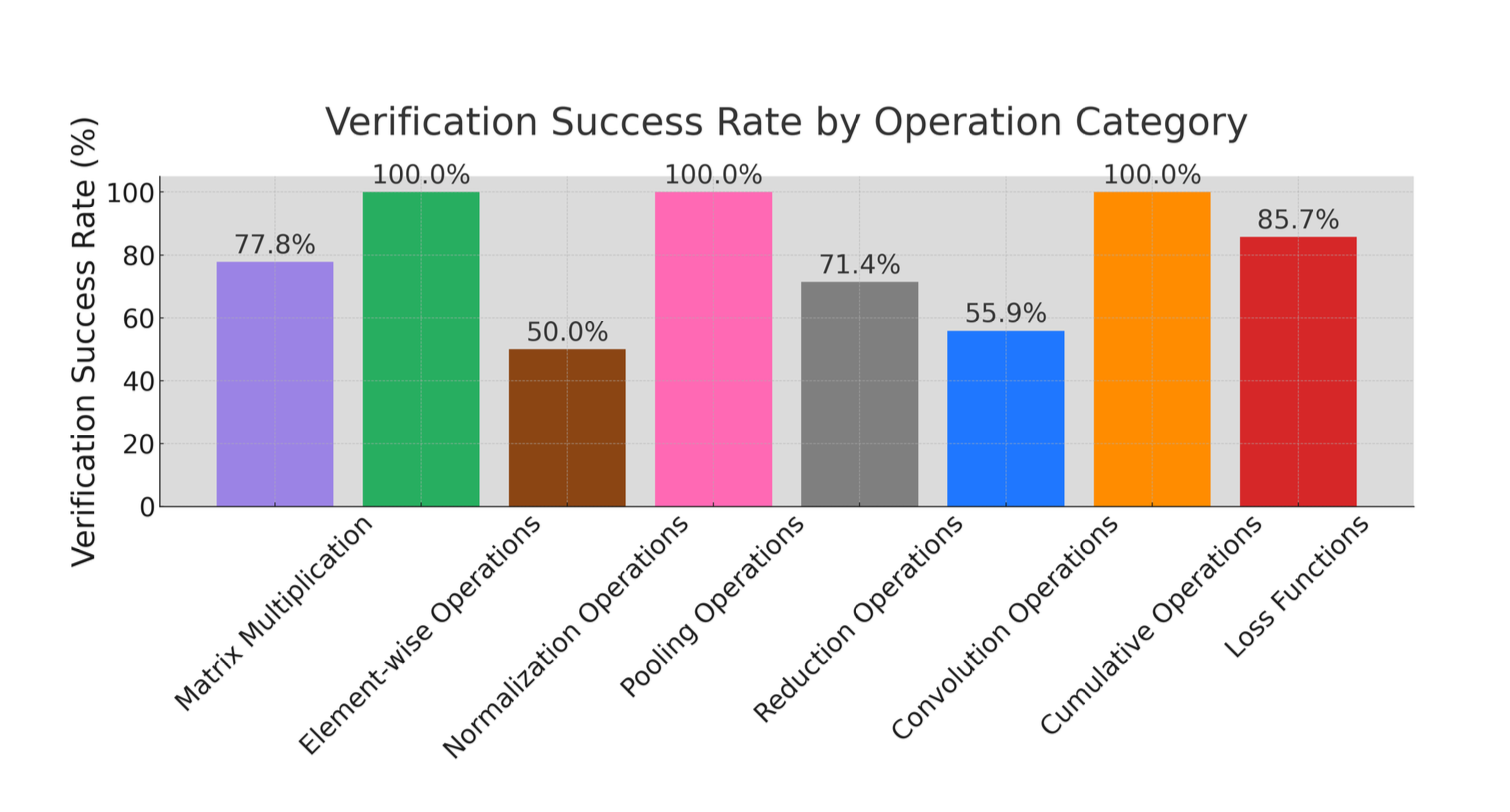
\includegraphics[width=0.6\textwidth]{figures/proofwright_figure.png}
    \caption{Verification coverage by operation category for the Claude-4-Sonnet baseline. The VerCors agent achieved full verification for element-wise, pooling, and cumulative operations, while matrix multiplication-based kernels exhibited partial coverage due to complex loop bounds and non-affine memory access patterns. Normalization and reduction operations showed moderate coverage. \textit{Figure reproduced from Chatterjee et al.} \cite{proofwright2025}.}
    \label{fig:proofwright-coverage}
\end{figure}

ProofWright verifies memory safety, thread safety, and semantic equivalence together for 14 CUDA kernels from KernelBench L1. The verified kernels follow a simple one-to-one parallel mapping pattern where each thread computes exactly one output element.

ProofWright performs verification via a VerCors agent that automatically inserts VerCors annotations in CUDA programs for formal verification. VerCors is a tool capable of verification of concurrent programs through annotations with functional properties and heap access permissions \cite{10.1007/978-3-319-06410-9_9}. The agent iteratively attempts to infer pre-conditions and post-conditions for a target kernel to annotate the CUDA kernel with VerCors. To do so, the agent must: (1) Identify all memory operations, (2) Identify whether each is read/write, (3) Describe memory locations and access conditions, and (4) Reason over synchronization/thread barriers. When the agent fails to generate verifiable annotations, it refines its annotations iteratively based on feedback, distilling knowledge in the dynamic VerCors Annotation Guide.

Over successive iterations, the agent develops the ability to classify kernels by algorithm family -- recognizing the memory access patterns, index-mapping schemes, and thread block configurations characteristic of each. This is directly relevant to our work: our benchmarks span five such families, and accurate family classification drives the verification strategies used by the agent.

Semantic equivalence checking proceeds in two stages. First, static analysis converts the PyTorch program into a graph-based IR where each node represents a computation and edges encode data dependencies. These nodes are then lifted into Rocq using MLRocq, a formal verification library that provides definitions for common deep learning operations -- including activation functions, loss functions, pooling, normalization, matrix operations, reductions, convolutions, and tensor manipulation. A semantic equivalence agent constructs Rocq theorems asserting that the lifted PyTorch representation matches the corresponding CUDA formalization in Rocq, and the proof is machine-checked. In the second stage, the agent derives VerCors functional annotations from the combined Rocq specifications and embeds them in the LLM-generated CUDA kernel; VerCors then discharges the resulting proof obligations via an SMT solver, confirming the kernel satisfies the original PyTorch specification.

Chatterjee et al. demonstrates that LLM-agent-driven Rocq verification is feasible for simple CUDA kernels, with the primary bottleneck being limited VerCors training data. Bridging this approach to C++ is harder than PyTorch due to the expressiveness of a general-purpose language, so we scope our effort to kernel-level equivalence across the five benchmark categories identified earlier. The following section presents a proof of concept using the Lean Theorem Prover and Claude Code.

\subsection{Experimenting with Claude Code and the Lean Theorem Prover}

Motivated by ProofWright's results, we investigated whether a similar approach could be applied to C++ kernels using the Lean Theorem Prover. A single Claude Code agent was given a CUDA matrix multiplication kernel and tasked with producing a Lean 4 definition capturing both the mathematical computation and the thread/memory access patterns, then proving it equal to the corresponding MathLib definition. We make two working assumptions: that a C++ kernel specification is already available (reasonable given that MACCHIATO employs ML methods to recognize and annotate code), and that the C++ source has already been independently verified. Mapping C++ to Lean in general remains an open research question; we treat it as out of scope here.

We chose matrix multiplication as our starting point because it is a clean one-to-one parallel mapping: each thread computes exactly one output element, threads collectively cover the entire output matrix, and their memory accesses are fully disjoint. ProofWright demonstrated equivalence for precisely this class of kernel but did not push beyond it. Our goal was to reproduce that baseline and then probe whether the approach extends to more complex mappings.

Figure~\ref{fig:lean-agent-prompt} shows the supplied Claude Code prompt. The referenced \texttt{expert.md} is an accumulated knowledge base. \texttt{tools/} is a directory of Lean 4 utilities made available to the agent: it includes MathLib (used to prove the agent's derived definition equivalent to the MathLib matrix multiplication) and a small bash script that invokes the Lean compiler to confirm that definitions and theorems typecheck and that all proof goals are closed. They can be found in the \href{https://github.com/cscaff/COMSE6901-Experiment-Repo/tree/main}{project repository} at \texttt{expert.md} and \texttt{tools/}, respectively. 

\begin{figure}[H]
\begin{promptbox}
You are an expert at understanding CUDA code and writing LEAN 4 code. Your goal is to do the following:

\medskip
Given the following CUDA kernel: \texttt{\{\{CUDA KERNEL CODE HERE\}\}}

\medskip
You will:
\begin{enumerate}
    \item Infer a mathematical mapping of the CUDA kernel. That mathematical definition must:
    \begin{itemize}
        \item Faithfully represent thread/memory semantics. Consider that different CUDA kernels have different thread/memory patterns: one-to-one mapping, stencil/diffusion, shared cache, reduction, iterative launch, etc.
        \item The mathematical model should represent that parallel pattern explicitly.
    \end{itemize}
    \item Translate and formalize the derived mathematical model into LEAN 4 using only the existing tools in \texttt{tools/} to verify that your translation is valid LEAN 4 code. The translated model must be valid LEAN 4 code. The model should not use Mathlib, only generic LEAN 4.
    \item Prove that the derived mathematical CUDA model is \textbf{functionally equal} to the MathLib Matrix Multiplication definition. That is, for all equal inputs into the CUDA LEAN definition and the MathLib definition, they both guarantee the exact same results. If you are unable to prove functional equality, return a LEAN counter example that proves the two functionally unequal.
    \item Store your learned knowledge about LEAN 4 and CUDA thread/memory patterns in \texttt{expert.md} such that you can use it as a knowledge-base in the future. Include known counter-examples you derive.
\end{enumerate}

\medskip
\textbf{Constraints:}
\begin{itemize}
    \item You must represent the CUDA kernel's thread/memory semantics as accurately to the source code as possible in your LEAN definition. You should never modify your LEAN definition in a manner that no longer represents the CUDA kernel in an attempt to prove equality.
    \item You may use knowledge from \texttt{expert.md}.
    \item You will never modify any files in \texttt{tools/}.
    \item You will output a JSON file in \texttt{outputs/} with the responses to the above instructions.
\end{itemize}

\medskip
\textbf{Example Output:}
\begin{minted}[fontsize=\small, breaklines]{json}
{
    "model": "Record model used",
    "prompt": "Record the given prompt here",
    "math_model": "response to 1",
    "lean_def": "response to 2",
    "theorem": "response to 3",
    "knowledge": "new knowledge from 4",
    "timing": "Record the time it took."
}
\end{minted}
\end{promptbox}
\caption{Claude Code agent prompt for CUDA-to-Lean formalization and equivalence proving.}
\label{fig:lean-agent-prompt}
\end{figure}

We then supplied the following kernel in Figure~\ref{fig:matmul-kernel}, deliberately omitting the call site to keep the initial experiment simple before increasing complexity.

\begin{figure}[H]
\begin{minted}[fontsize=\scriptsize, breaklines, frame=single]{C++}
__global__ void matMulKernel(int* A, int* B, int* C, int N) {
    int row = blockIdx.y * blockDim.y + threadIdx.y;
    int col = blockIdx.x * blockDim.x + threadIdx.x;

    if (row < N && col < N) {
        int sum = 0;

       for (int k = 0; k < N; ++k)
            sum += A[row * N + k] * B[k * N + col];
            C[row * N + col] = sum;
    }
}
\end{minted}
\caption{CUDA matrix multiplication kernel supplied to the Claude Code agent.}
\label{fig:matmul-kernel}
\end{figure}

\subsection{Claude Code Results}

Below, we illustrate the results of the experiment. Claude Code successfully mapped the CUDA kernel to a Lean definition that conveyed thread semantics. The agent was able to prove this definition functionally equivalent to the MathLib matrix multiplication definition, returning a JSON as instructed that contained the following: (1) LLM model (2) prompt summary (3) math model (4) Lean definition (5) theorem of equivalence (6) derived knowledge (7) timing.

\begin{figure}[H]
\begin{promptbox}
Claude Sonnet 4.6
\end{promptbox}
\caption{LLM model used for the Lean equivalence experiment.}
\label{fig:lean-model}
\end{figure}

\begin{figure}[H]
\begin{promptbox}
Given the following CUDA kernel:

\begin{minted}[fontsize=\small, breaklines]{cuda}
__global__ void matMulKernel(int* A, int* B, int* C, int N) {
    int row = blockIdx.y * blockDim.y + threadIdx.y;
    int col = blockIdx.x * blockDim.x + threadIdx.x;
    if (row < N && col < N) {
        int sum = 0;
        for (int k = 0; k < N; ++k)
            sum += A[row * N + k] * B[k * N + col];
            C[row * N + col] = sum;
    }
}
\end{minted}

You will:
\begin{enumerate}
    \item Infer a mathematical mapping of the CUDA kernel.
    \item Translate and formalize the derived mathematical model into LEAN 4.
    \item Prove that the derived mathematical CUDA model is \textbf{functionally equal} to the MathLib Matrix Multiplication definition.
    \item Store learned knowledge in \texttt{expert.md}.
\end{enumerate}
\end{promptbox}
\caption{Claude Code's summarization of the supplied prompt.}
\label{fig:lean-prompt-summary}
\end{figure}

\paragraph{Mathematical Model}

The LLM derived the following model in Figure~\ref{fig:lean-math-model}, noting the threads communicated a one-to-one parallel mapping where if-guards enforced a finite set.

\begin{figure}[H]
\begin{promptbox}
\textbf{Pattern}: One-to-One Output-Parallel

\medskip
Thread index mapping (global 2D grid):
\begin{minted}[fontsize=\small, breaklines]{cuda}
row = blockIdx.y * blockDim.y + threadIdx.y
col = blockIdx.x * blockDim.x + threadIdx.x
\end{minted}

\medskip
\textbf{Domain}: \texttt{row, col} $\in$ \texttt{Fin N} (i.e., $[0, N)$ enforced by the if-guard)

\medskip
Each thread \texttt{(row, col)} owns exactly one output element and computes:
$$C(\text{row}, \text{col}) := \sum_{k \in \text{Fin } N} A(\text{row}, k) \times B(k, \text{col})$$
\end{promptbox}
\caption{Claude Code's derived mathematical model: thread mapping, domain, and per-thread computation.}
\label{fig:lean-math-model}
\end{figure}

An interesting note is that the LLM entirely ignores the representation of a flat 1D array, opting to model the matrix as a 2D array. LLMs are susceptible to this kind of issue due to a lack of deterministic behavior, necessitating careful prompting for correctness. The prompt should have communicated that the LLM needs to respect indexing schemes.

Next, the LLM focused on the parallel semantics in Figure~\ref{fig:lean-parallel-semantics}, noting the principal idea that the mapping is bijective -- each thread maps to a unique output.

\begin{figure}[H]
\begin{promptbox}
\textbf{Parallel semantics:}
\begin{itemize}
    \item The thread-to-output mapping is bijective: $N^2$ threads $\rightarrow$ $N^2$ distinct output positions.
    \item No inter-thread communication (no \texttt{\_\_shared\_\_} memory, no \texttt{\_\_syncthreads}).
    \item Memory access: thread \texttt{(row, col)} reads all of \texttt{A[row, *]} (global) and all of \texttt{B[*, col]} (global).
    \item Inner loop \texttt{for k = 0..N-1} is a sequential accumulation within a single thread:
    \texttt{sum = 0; for each k: sum = sum + A[row,k]*B[k,col]}. This is a left-associative accumulation: $((0 + f(0)) + f(1)) + \ldots + f(N-1)$.
\end{itemize}
\end{promptbox}
\caption{Claude Code's analysis of the kernel's parallel semantics.}
\label{fig:lean-parallel-semantics}
\end{figure}

Figure~\ref{fig:lean-formal-model} shows the formal model derived, illustrating:

\begin{enumerate}
    \item A matrix as a function that takes rows and columns and outputs an integer.
    \item A matrix multiplication function that computes a specific entry as:
    $$\sum_{k \in N} A(\mathrm{row}, k) \times B(k, \mathrm{col})$$
\end{enumerate}

\begin{figure}[H]
\begin{promptbox}
\textbf{Formal model:}
$$\text{Let } A, B : \text{Fin } N \rightarrow \text{Fin } N \rightarrow \mathbb{Z}$$
$$\text{cudaMatMulKernel}(A, B) := \lambda\ \text{row}\ \text{col}.\ \sum_{k \in \text{Fin } N} A(\text{row}, k) \times B(k, \text{col})$$
where $\Sigma$ is a left-fold (matching the sequential CUDA accumulation).
\end{promptbox}
\caption{Claude Code's formal mathematical model of the CUDA matrix multiplication kernel.}
\label{fig:lean-formal-model}
\end{figure}

\paragraph{Lean Definition}

The LLM synthesized a Lean definition, ensuring it compiled via a bashscript in \texttt{tools/}.

\begin{figure}[H]
\begin{minted}[fontsize=\small, breaklines, frame=single]{lean}
-- isum models the CUDA inner for-loop: sum = 0; for k in [0,N): sum += f(k)
-- Left-recursive: isum n f = isum (n-1) f' + f(n-1), unfolding to ((0+f(0))+f(1))+...+f(n-1)
def isum : (n : Nat) → (Fin n → Int) → Int
  | 0, _ => 0
  | n + 1, f =>
    isum n (fun i => f ⟨i.val, Nat.lt_succ_of_lt i.isLt⟩) +
    f ⟨n, Nat.lt_succ_self n⟩
\end{minted}
\caption{Lean 4 \texttt{isum} definition modeling the CUDA inner accumulation loop.}
\label{fig:lean-isum}
\end{figure}

The LLM represented the inner CUDA \texttt{for}-loop that occurs over $k$ iterations in Figure~\ref{fig:lean-isum}. The definition receives the following inputs: (1) A natural number \texttt{n} and (2) A function \texttt{f} defined on \texttt{n} indices. The definition computes one integer result, is recursive with a base case that returns 0 when \texttt{n = 0}, and recurses on \texttt{n + 1} by applying \texttt{isum} recursively and adding the inductive step.

The agent then builds the full kernel definition in three steps. First, it introduces a \texttt{CudaMatrix} type alias that models an $N \times N$ integer matrix as a curried function over \texttt{Fin N} indices (figure~\ref{fig:lean-cudamatrix}). It then defines \texttt{cudaThreadCompute}, which captures the computation of a single thread \texttt{(row, col)}: it calls \texttt{isum} with the function $k \mapsto A(\mathrm{row}, k) \times B(k, \mathrm{col})$, directly encoding $\sum_{k \in \text{Fin}\,N} A(\mathrm{row}, k) \times B(k, \mathrm{col})$ (figure~\ref{fig:lean-threadcompute}). Finally, \texttt{cudaMatMulKernel} lifts the per-thread computation to the full matrix by mapping \texttt{cudaThreadCompute} over all output positions, reflecting the one-to-one parallel structure of the kernel (figure~\ref{fig:lean-matmulkernel}).

\begin{figure}[H]
\begin{minted}[fontsize=\small, breaklines, frame=single]{lean}
-- N×N integer matrix as a function (matches CUDA int* with row-major indexing)
abbrev CudaMatrix (N : Nat) := Fin N → Fin N → Int
\end{minted}
\caption{Lean 4 \texttt{CudaMatrix} type alias modeling an $N \times N$ integer matrix.}
\label{fig:lean-cudamatrix}
\end{figure}

\begin{figure}[H]
\begin{minted}[fontsize=\small, breaklines, frame=single]{lean}
-- Thread (row, col) computes its single output element
-- One-to-one pattern: each thread independently owns C[row,col]
def cudaThreadCompute (N : Nat) (A B : CudaMatrix N) (row col : Fin N) : Int :=
  isum N (fun k => A row k * B k col)
\end{minted}
\caption{Lean 4 \texttt{cudaThreadCompute}: per-thread dot-product computation.}
\label{fig:lean-threadcompute}
\end{figure}

\begin{figure}[H]
\begin{minted}[fontsize=\small, breaklines, frame=single]{lean}
-- Full kernel: all threads execute in parallel, each writing to a distinct C[i,j]
def cudaMatMulKernel (N : Nat) (A B : CudaMatrix N) : CudaMatrix N :=
  fun row col => cudaThreadCompute N A B row col

-- Verified eval: 1×1 → 12, 2×2 → (19, 22, 43, 50) ✓
\end{minted}
\caption{Lean 4 \texttt{cudaMatMulKernel}: full matrix multiplication lifting per-thread computation.}
\label{fig:lean-matmulkernel}
\end{figure}

\paragraph{Proving Equality Between the CUDA Matrix Multiply and MathLib's Matrix Multiplication}

\begin{figure}[H]
\begin{minted}[fontsize=\small, breaklines, frame=single]{lean}
-- Bridge lemma: the sequential CUDA loop equals Mathlib's abstract Finset.sum
lemma isum_eq_finset_sum (n : Nat) (f : Fin n → Int) :
    isum n f = ∑ k : Fin n, f k := by
  induction n with
  | zero => simp [isum]
  | succ n ih =>
    simp only [isum, Fin.sum_univ_castSucc]
    have h_cast : ∀ i : Fin n,
        f ⟨i.val, Nat.lt_succ_of_lt i.isLt⟩ = f (Fin.castSucc i) :=
      fun i => congr_arg f (Fin.ext rfl)
    have h_last : f ⟨n, Nat.lt_succ_self n⟩ = f (Fin.last n) :=
      congr_arg f (Fin.ext rfl)
    simp_rw [h_cast, h_last, ih]
\end{minted}
\caption{Lean 4 bridge lemma proving \texttt{isum} equivalent to Mathlib's \texttt{Finset.sum}.}
\label{fig:lean-isum-bridge}
\end{figure}

Figure~\ref{fig:lean-isum-bridge} proves that \texttt{isum} agrees with Mathlib's \texttt{Finset.sum}, i.e.\ $\text{isum}(n, f) = \sum_{k \in \text{Fin}\,n} f(k)$. The proof proceeds by induction: the base case is discharged by \texttt{simp}, and for the inductive step \texttt{simp only [isum, Fin.sum\_univ\_castSucc]} expands both sides into $\bigl(\sum_{i \in \text{Fin}(n)} f(\text{castSucc}\,i)\bigr) + f(\text{last})$. Two auxiliary facts — \texttt{h\_cast} and \texttt{h\_last} — then align the \texttt{isum} indices with Mathlib's \texttt{castSucc}/\texttt{last} representation via \texttt{Fin.ext rfl}, after which \texttt{simp\_rw} closes the goal using those equalities together with the inductive hypothesis.

\begin{figure}[H]
\begin{minted}[fontsize=\small, breaklines, frame=single]{lean}
-- Main theorem: CUDA kernel is functionally equal to Mathlib Matrix.mul
theorem cudaMatMul_eq_mathlib (N : Nat) (A B : Matrix (Fin N) (Fin N) Int) :
    cudaMatMulKernel N A B = A * B := by
  funext row col
  simp only [cudaMatMulKernel, cudaThreadCompute, Matrix.mul_apply]
  exact isum_eq_finset_sum N (fun k => A row k * B k col)

-- Result: PROVEN FUNCTIONALLY EQUAL for all N and all integer matrices A, B.
\end{minted}
\caption{Lean 4 theorem proving \texttt{cudaMatMulKernel} functionally equal to Mathlib's \texttt{Matrix.mul} for all $N$ and all integer matrices.}
\label{fig:lean-main-theorem}
\end{figure}

The theorem shown in Figure~\ref{fig:lean-main-theorem} proves the two definitions equal by proving each product matrix entry equal for all inputs. \texttt{simp} expands the definitions, reducing the goal to proving \texttt{isum} holds for \texttt{fun k => A row k * B k col}, which is discharged by \texttt{isum\_eq\_finset\_sum}.

\paragraph{Knowledge Base Update}

The LLM updated \texttt{expert.md} with the following knowledge base entry in Figure~\ref{fig:lean-expert-knowledge}.

\begin{figure}[H]
\begin{promptbox}
\begin{enumerate}
    \item \textbf{CUDA ONE-TO-ONE PATTERN}: \texttt{matMulKernel} is one-to-one output-parallel — each thread maps bijectively to one output cell, no shared memory or reduction. Lean model: \texttt{$\lambda$ row col. isum N (fun k => A row k * B k col)}.

    \item \textbf{\texttt{isum} models the CUDA loop}: Define \texttt{isum} recursively, adding the last element at each step. This gives left-associative accumulation matching \texttt{sum += f(k)} for \texttt{k=0..N-1}.

    \item \textbf{Bridge lemma}: \texttt{isum n f = $\sum$ k : Fin n, f k}. Proved by induction using \texttt{Fin.sum\_univ\_castSucc}, which splits $\sum_{i : \text{Fin}(n+1)} f(i)$ into $(\sum_{i : \text{Fin}(n)} f(\text{castSucc}\ i)) + f(\text{last})$. Use \texttt{simp\_rw} (not \texttt{simp only}) to rewrite under binders.

    \item \textbf{\texttt{Fin} equality}: \texttt{Fin.ext rfl} proves $\langle i.\text{val}, h_1\rangle = \text{Fin.castSucc}\ i$ and $\langle n, \_\rangle = \text{Fin.last}\ n$. Use \texttt{congr\_arg f (Fin.ext rfl)} to lift to function applications.

    \item \textbf{Matrix type annotation}: For \texttt{Matrix.mul\_apply} to fire in \texttt{simp}, arguments must be typed as \texttt{Matrix (Fin N) (Fin N) Int}, not as \texttt{Fin N $\rightarrow$ Fin N $\rightarrow$ Int}, even though they are definitionally equal.

    \item \textbf{No counter-examples}: \texttt{cudaMatMulKernel} is genuinely equal to \texttt{Matrix.mul} over \texttt{Int}. Divergence would occur only if modeling 32-bit overflow or if the thread-bound guard were removed.
\end{enumerate}
\end{promptbox}
\caption{Knowledge distilled by the agent into \texttt{expert.md} after the matrix multiplication experiment.}
\label{fig:lean-expert-knowledge}
\end{figure}

The LLM completed the task in 6 minutes and 20 seconds.

\subsection{Experiment with Dot Products}

Given how well the LLM performed on matrix multiplication, we expand to the dot product kernel.

\begin{figure}[H]
\begin{minted}[fontsize=\small, breaklines, frame=single]{cuda}
__global__ void dotProductKernel(float* A, float* B, float* partial, int n) {
    __shared__ float cache[256];
    int tid = blockIdx.x * blockDim.x + threadIdx.x;
    int cacheIndex = threadIdx.x;
    float temp = 0.0f;
    while (tid < n) {
        temp += A[tid] * B[tid];
        tid += blockDim.x * gridDim.x;
    }
    cache[cacheIndex] = temp;
    __syncthreads();
    for (int i = blockDim.x / 2; i > 0; i >>= 1) {
        if (cacheIndex < i) cache[cacheIndex] += cache[cacheIndex + i];
        __syncthreads();
    }
    if (cacheIndex == 0) partial[blockIdx.x] = cache[0];
}
\end{minted}
\caption{CUDA dot product kernel using shared memory and a parallel tree reduction.}
\label{fig:dot-product-kernel}
\end{figure}

However, the LLM timed out after $\sim 20$ minutes without any output. More complex memory patterns such as tree reduction and shared cache are significantly more difficult for the LLM to reason about.  

\section{Conclusion}

MACCHIATO is a novel end-to-end compiler tool-chain that aims to overcome challenges in reducing human effort to refactor and optimize code for platforms based on heterogeneous compute elements through machine learning (ML) and language models (LMs) \cite{HR001124S0035}. Within this work, we focus our efforts on program equivalence, an important component in verifying the LLM-based rewrites that occur in the MACCHIATO compiler tool-chain. We demonstrate how one, unfamiliar with the problem, might approach it. Then we present two core experiments: (1) a CBMC-backed approach and (2) an agentic approach with the Lean interactive theorem prover. 

\newpage

\printbibliography[heading=bibintoc, title={References}]

\end{document}